% $Header: /Users/joseph/Documents/LaTeX/beamer/solutions/generic-talks/generic-ornate-15min-45min.en.tex,v 90e850259b8b 2007/01/28 20:48:30 tantau $

\documentclass[handout]{beamer}
\usepackage{pgfpages}
\pgfpagesuselayout{4 on 1}[a4paper,border shrink=5mm,landscape]


\mode<presentation>
{
  \usetheme{cambridge}
  %\usetheme{Warsaw}

  \setbeamertemplate{navigation symbols}{}
  \setbeamercovered{transparent}
  % or whatever (possibly just delete it)
}

\usepackage[english]{babel}
\usepackage[latin1]{inputenc}
\usepackage{multicol}

%\usepackage{times}
%\usepackage[T1]{fontenc}
% Or whatever. Note that the encoding and the font should match. If T1
% does not look nice, try deleting the line with the fontenc.


\title[HPC: An introduction] % (optional, use only with long paper titles)
{An Introduction to High Performance Computing}

%\subtitle
%{Presentation Subtitle} % (optional)

\author[SJ Rankin] % (optional, use only with lots of authors)
{Stuart Rankin\\ \texttt{sjr20@cam.ac.uk}}
%{F.~Author\inst{1} \and S.~Another\inst{2}}
% - Use the \inst{?} command only if the authors have different
%   affiliation.

\institute[Research Computing Services, University of Cambridge] % (optional, but mostly needed)
{Research Computing Services (http://www.hpc.cam.ac.uk/)\\
University Information Services (http://www.uis.cam.ac.uk/)}
% - Use the \inst command only if there are several affiliations.
% - Keep it simple, no one is interested in your street address.

\date[20/06/2019] % (optional)
{20th June 2019 / UIS Training}

\subject{Courses}


\begin{document}

\begin{frame}
  \titlepage
\end{frame}

\begin{frame}<presentation>{Welcome}
\begin{itemize}
\item{Please sign in on the {\color{red}attendance sheet}.}
\item Please give your {\color{red}online feedback} at the end of the course:
      \url{http://feedback.training.cam.ac.uk/ucs/form.php}
\item{Keep your belongings with you.}
%\item Course files can be downloaded from:  \url{www.ucs.cam.ac.uk/training/files}
\item\alert{Please ask questions and let us know if you need assistance.}
\end{itemize}
\end{frame}

\section{Who are we?}
\begin{frame}{UIS: Research Computing Services}
Your trainers for today will be:\\
\begin{itemize}
\item{\alert{Stuart Rankin}\\{}\qquad\qquad Research Computing User Services}
\item{\alert{Mark Sharpley}\\{}\qquad\qquad Research Computing Platforms}
\item{We are generalists, but there is also the \alert{Research Software Engineering} team.}
\end{itemize}
\end{frame}

\section{Who are you?}
\begin{frame}{You may be $\ldots$}
  \begin{itemize}
  \item{Programmers (or not).}\pause
  \item{UNIX power users (or not).}\pause
  \item{Researchers wishing to run large, parallel code.}\pause
  \item{Researchers wishing to run many, non-parallel cases.}\pause
  \item{Researchers interested in big data, machine learning, AI.}\pause
  \item{Researchers requiring slightly more than an ordinary workstation.}\pause
  \item{\alert{Many different disciplines and requirements.}}
\end{itemize}
\end{frame}


\begin{frame}<presentation>{Plan of the Course}
\begin{description}
\item[Part 1:]{Basics}
\item[Part 2:]{Research Computing Services HPC}
\item[Part 3:]{Using HPC}
\end{description}
\end{frame}

\section{Prerequisites}
\begin{frame}{Prerequisites}
\begin{itemize}
\item{Basic Unix/Linux command line experience:\hfill\break
\alert{Unix: Introduction to the Command Line Interface (self-paced)}\hfill\break \small\url{https://www.training.cam.ac.uk/ucs/Course/ucs-unixintro1}}
\pause
\item{Shell scripting experience is desirable:\hfill\break
\alert{Unix: Simple Shell Scripting for Scientists}\hfill\break  \small\url{https://www.training.cam.ac.uk/ucs/Course/ucs-scriptsci}}
\end{itemize}
\end{frame}

\section{Training Accounts}
\begin{frame}{Training accounts}
\begin{itemize}
\item{\alert{For our practical exercises we will use HPC training accounts.} These are distinct from the MCS desktop training accounts.}
\pause
\item{You will find HPC training account details on your desk.}
\pause
\item{Your HPC training account is valid only for today.}
\pause
\item{The name of the HPC account will be the same as your MCS desktop account: z4\alert{XY} (where \alert{XY} is the station number).}
\item{Please check your MCS workstation is booted into Ubuntu Linux, and logged in, ask if you need help with this.}
\item{PDFs of the course notes and the exercises can be found in your MCS filespace.}
\end{itemize}
\end{frame}

\section{Security}
\begin{frame}{Security}
\begin{itemize}
\item{Cambridge IT is under constant attack by would-be intruders.}
\pause
\item{\alert{Choose strong passwords and keep it (or private key passphrase) safe.}}
\pause
\item{\alert{Your UIS password is used for multiple systems so keep it secure!}}
\pause
\item{Keep the software on your laptops/tablets/PCs up to date --- this includes home computers.}
  \pause
\item{Check out and install free anti-malware software available for work and home:\hfill
  \null\qquad\alert{\small https://help.uis.cam.ac.uk/service/security/stay-safe-online/malware}}
  \pause
\item{Don't share accounts (this is against the rules, and anyone can get their own).}
\end{itemize}
\end{frame}


\part{Basics}
\frame{\partpage}

\section{Why Buy a Big Computer?}

\begin{frame}{Basics: Why Buy a Big Computer?}
  % - A title should summarize the slide in an understandable fashion
  %   for anyone how does not follow everything on the slide itself.

What types of big problem might require a ``Big Computer''?

\begin{description}
\pause
\item[\textit{Compute Intensive:}]{A single problem requiring a large amount of computation.}
\pause
\item[\textit{Memory Intensive:}]{A single problem requiring a large amount of memory.}
\pause
\item[\textit{Data Intensive:}]{A single problem operating on a large amount of data.}
\pause
\item[\textit{High Throughput:}]{Many unrelated problems to be executed in bulk.}
\end{description}
\end{frame}

\begin{frame}{Basics: Compute Intensive Problems}
\begin{itemize}
\item{Distribute the \alert{work} for a \alert{single problem} across multiple CPUs to reduce the execution time as far as possible.}
\pause
\item{Program workload must be \emph{parallelised}:}
\begin{description}
\item{Parallel programs split into copies (processes or threads).}
\item{Each process/thread performs a part of the work on its own CPU, concurrently with the others.}
\item{A well-parallelised program will fully exercise as many CPUs as there are processes/threads.}
\end{description}
\pause
\item{The CPUs typically need to exchange information rapidly, requiring specialized communication hardware.}
\pause
\item{Many use cases from Physics, Chemistry, Engineering, Astronomy, Biology...}
\item{The traditional domain of \alert{HPC} and the \alert{Supercomputer}.}
\end{itemize}
\end{frame}

\begin{frame}{Basics: Scaling \& Amdahl's Law}
\begin{itemize}
\item{\alert{Using more CPUs is not necessarily faster.}}
  \pause
\item{Typically parallel codes have a \alert{scaling limit}.}
\item{Partly due to the system overhead of managing more copies, but also to more basic constraints;}
\pause
\item{Amdahl's Law (idealized):}
\[
S(N)=\frac{1}{\left(1-p+\frac{p}{N}\right)}
\]
where \begin{align*}S(N)&\text{ is the fraction by which the program has sped up}\\&\text{ relative to $N=1$}\\
p&\text{ is the fraction of the program which can be parallelized}\\
N&\text{ is the number of CPUs.}
\end{align*}
\end{itemize}
\end{frame}

\begin{frame}{Basics: Amdahl's Law}
\centerline{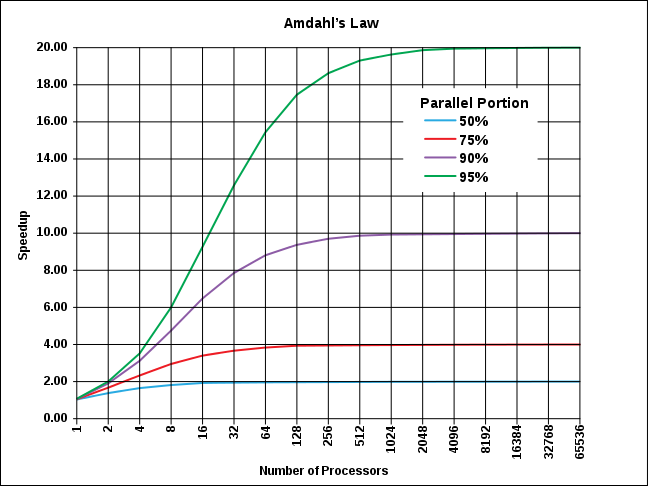
\includegraphics[width=0.75\textwidth]{imgs/AmdahlsLaw.png}}%
\rightline{\tiny http://en.wikipedia.org/wiki/File:AmdahlsLaw.svg}
\smallskip
\end{frame}

\begin{frame}{The Bottom Line}
\begin{itemize}
\item{Parallelisation requires effort:}
\begin{itemize}
\item{There are libraries to help (e.g. \alert{OpenMP}, \alert{MPI}).}
\item{Aim to make both $p$ and performance per CPU as large as possible.}
\end{itemize}
\pause
\item{The scaling limit: eventually using more CPUs becomes \alert{detrimental} instead of helpful.}
\end{itemize}
\end{frame}

\begin{frame}{Basics: Data Intensive Problems}
\begin{itemize}
\item{Distribute the \alert{data} for a \alert{single problem} across multiple CPUs to reduce the overall execution time.}
\pause
\item{The \emph{same} work may be done on each data segment.}
\pause
\item{Rapid movement of data to and from disk is more important than inter-CPU communication.}
\pause
\item{\alert{Big Data} problems of great current interest -}
\item{Hadoop/MapReduce}
\item{Life Sciences (genomics) and elsewhere.}
\end{itemize}
\end{frame}

\begin{frame}{Basics: High Throughput}
\begin{itemize}
\item{Distribute \alert{independent}, \alert{multiple problems} across multiple CPUs to reduce the overall execution time.}
\pause
\item{Workload is trivially (or \emph{embarrassingly}) parallel:}
\begin{itemize}
\item[$\ast$]{Workload breaks up naturally into \emph{independent} pieces.}
\item[$\ast$]{Each piece is performed by a separate process/thread on a separate CPU (concurrently).}
\item[$\ast$]{\alert{Little or no inter-CPU communication}.}
\end{itemize}
\pause
\item{Emphasis is on throughput over a period, rather than on performance on a single problem.}
\pause
\item{Compute intensive capable $\Rightarrow$ high throughput capable (not conversely).}
\end{itemize}
\visible<5->{If you are using lots of R or python, you are \alert{probably} high throughput, and \alert{possibly} data intensive or compute intensive.}
\end{frame}

%\begin{frame}{Basics: Memory Intensive Problems}
%\begin{itemize}
%\item{Require aggregation of large memory, rather than many CPUs.}
%\pause
%\begin{description}
%\item{\alert{NB Memory (fast, volatile) not disk (slow, non-volatile).}}
%\end{description}
%\pause
%\item{Performance optimisation is harder (memory layout tends to be highly nonuniform).}   
%  \pause
%\item{More technically difficult and expensive to scale beyond a single box.}   
%  \pause
%\item{If you think you have a memory intensive problem, are you sure it needs to be?}
%\end{itemize}
%\end{frame}

\begin{frame}{Basics: Putting it All Together}
\begin{itemize}
\item{Each of these types of problem requires \alert{combining many CPUs and memory modules}.}
\pause
\item{Nowadays, there can be many CPUs and memory modules inside a \alert{single commodity PC or server}.}
  \pause
\item{HPC involves combining \alert{many times more than this}.}
\end{itemize}
\end{frame}
 

%Tasks may be small or large, uniprocessor or multiprocessor, compute-intensive or data-intensive. The set of tasks may be static or dynamic, homogeneous or heterogeneous, loosely coupled or tightly coupled.

%large volumes TB or PB of data and devote most of their processing time to I/O and manipulation of data are deemed data-intensive
%data parallel: concurrent processing of different pieces of data
%big data!
%Compute intensive: Task parallel: concurrent processing of different threads of execution
%embarrassingly parallel: little or no effort is required to separate the problem into a number of parallel tasks
%Amdahl

%If the communication overhead of additional processors outweighs the benefit of adding another processor, one encounters parallel slowdown.

%Condor HTC:  environments that can deliver large amounts of processing capacity over long periods of time. We refer to such environments as High Throughput Computing (HTC) environments.

%The European Grid Infrastructure defines HTC as “a computing paradigm that focuses on the efficient execution of a large number of loosely-coupled tasks. Given the minimal parallel communication requirements, the tasks can be executed on clusters or physically distributed resources using grid technologies. HTC systems are typically optimised to maximise the throughput over a long period of time and a typical metric is jobs per month or year.
%HPC: focuses on the efficient execution of compute intensive, tightly-coupled tasks. Given the high parallel communication requirements, the tasks are typically executed on low latency interconnects which makes it possible to share data very rapidly between a large numbers of processors working on the same problem.''

%Grid computing: distributed, heterogeneous environment that supports collections of users and resources (Virtual Organisations) across traditional administrative, trust and organisational boundaries (real organisations).''

%Integration

%Supercomputer: A supercomputer is a computer at the frontline of contemporary processing capacity – particularly speed of calculation which can happen at speeds of nanoseconds.

%capacity vs capability

%Top500

\section{Inside a Modern Computer}
\begin{frame}{Basics: Inside a Modern Computer}{CPUs in a box}
\only<1-7>{%
\begin{itemize}
\item<1-7>{Today's commodity servers already aggregate both CPUs and memory to make a \alert{single system image} in a single box.}
\item<2-7>{Even small computers now have multiple \alert{cores} (fully functional CPUs) per socket.}%\hfill\\
%\visible<3-7>{\alert{$\implies{}$each socket (plus its local memory) is a Symmetric Multi-Processor (SMP)}.}}
\item<3-7>{Larger computers have multiple sockets (each with their own local memory).%:\hfill\\
%{}\qquad \visible<4-7>{all CPUs (unequally) share the node memory\hfill}\\
%{}\qquad \visible<5-7>{$\implies{}$the node is a \alert{shared memory} multiprocessor}\\
%{}\qquad \visible<6-7>{with Non-Uniform Memory Architecture (\alert{NUMA})}\\
  %{}\qquad \visible<7>{but users still see a single computer (\alert{single system image}).}%
}
\end{itemize}
}%
\end{frame}

\begin{frame}{Basics: Inside a Modern Computer}{CPUs in a box}
\centerline{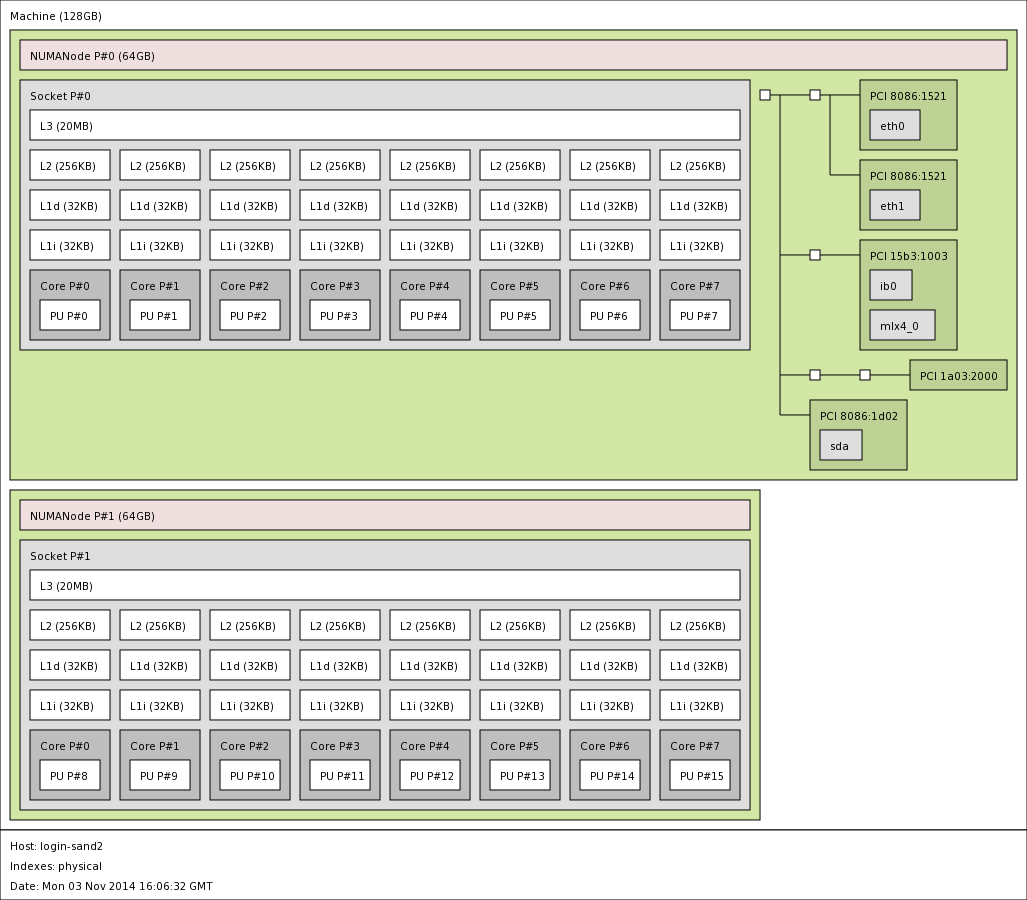
\includegraphics[width=0.8\textwidth]{imgs/lstopo.png}}
\end{frame}

\section{How to Build a Supercomputer}
\begin{frame}{Basics: How to Build a Supercomputer}
\only<1,2>{\begin{itemize}
\item{A supercomputer aggregates contemporary CPUs and memory to obtain increased computing power.}
\pause
\item{Usually today these are \alert{clusters}.}
\end{itemize}}
\only<3->{\begin{enumerate}
\item{Take some (multicore) processors plus some memory to make a \alert{node}.}
\begin{itemize}
\item<4->{Could be an off-the-shelf server, or something more special.}
%\item<5->{A NUMA, shared memory, multiprocessor building block: a \alert{node}.}
\end{itemize}
\end{enumerate}
}
\end{frame}


\begin{frame}{Basics: How to Build a Supercomputer}
\begin{tabular}{ll}
\parbox[c]{0.5\textwidth}{\begin{enumerate}
\setcounter{enumi}{1}
\item{Connect similar nodes with one or more \alert{networks}. E.g.}
\begin{description}
\item[Gbit Ethernet:]{\alert{100 MB/sec}}
\item[Omni-Path:]{\alert{10 GB/sec}}
\end{description}
\pause
\null\par
Faster network is for \alert{inter-CPU communication across nodes}.\par
Slower network is for \alert{management} and \alert{provisioning}.\par
\alert{Storage} may use either.
\end{enumerate}}
&\vbox to 0pt{\vss\vskip 0.25cm\leftline{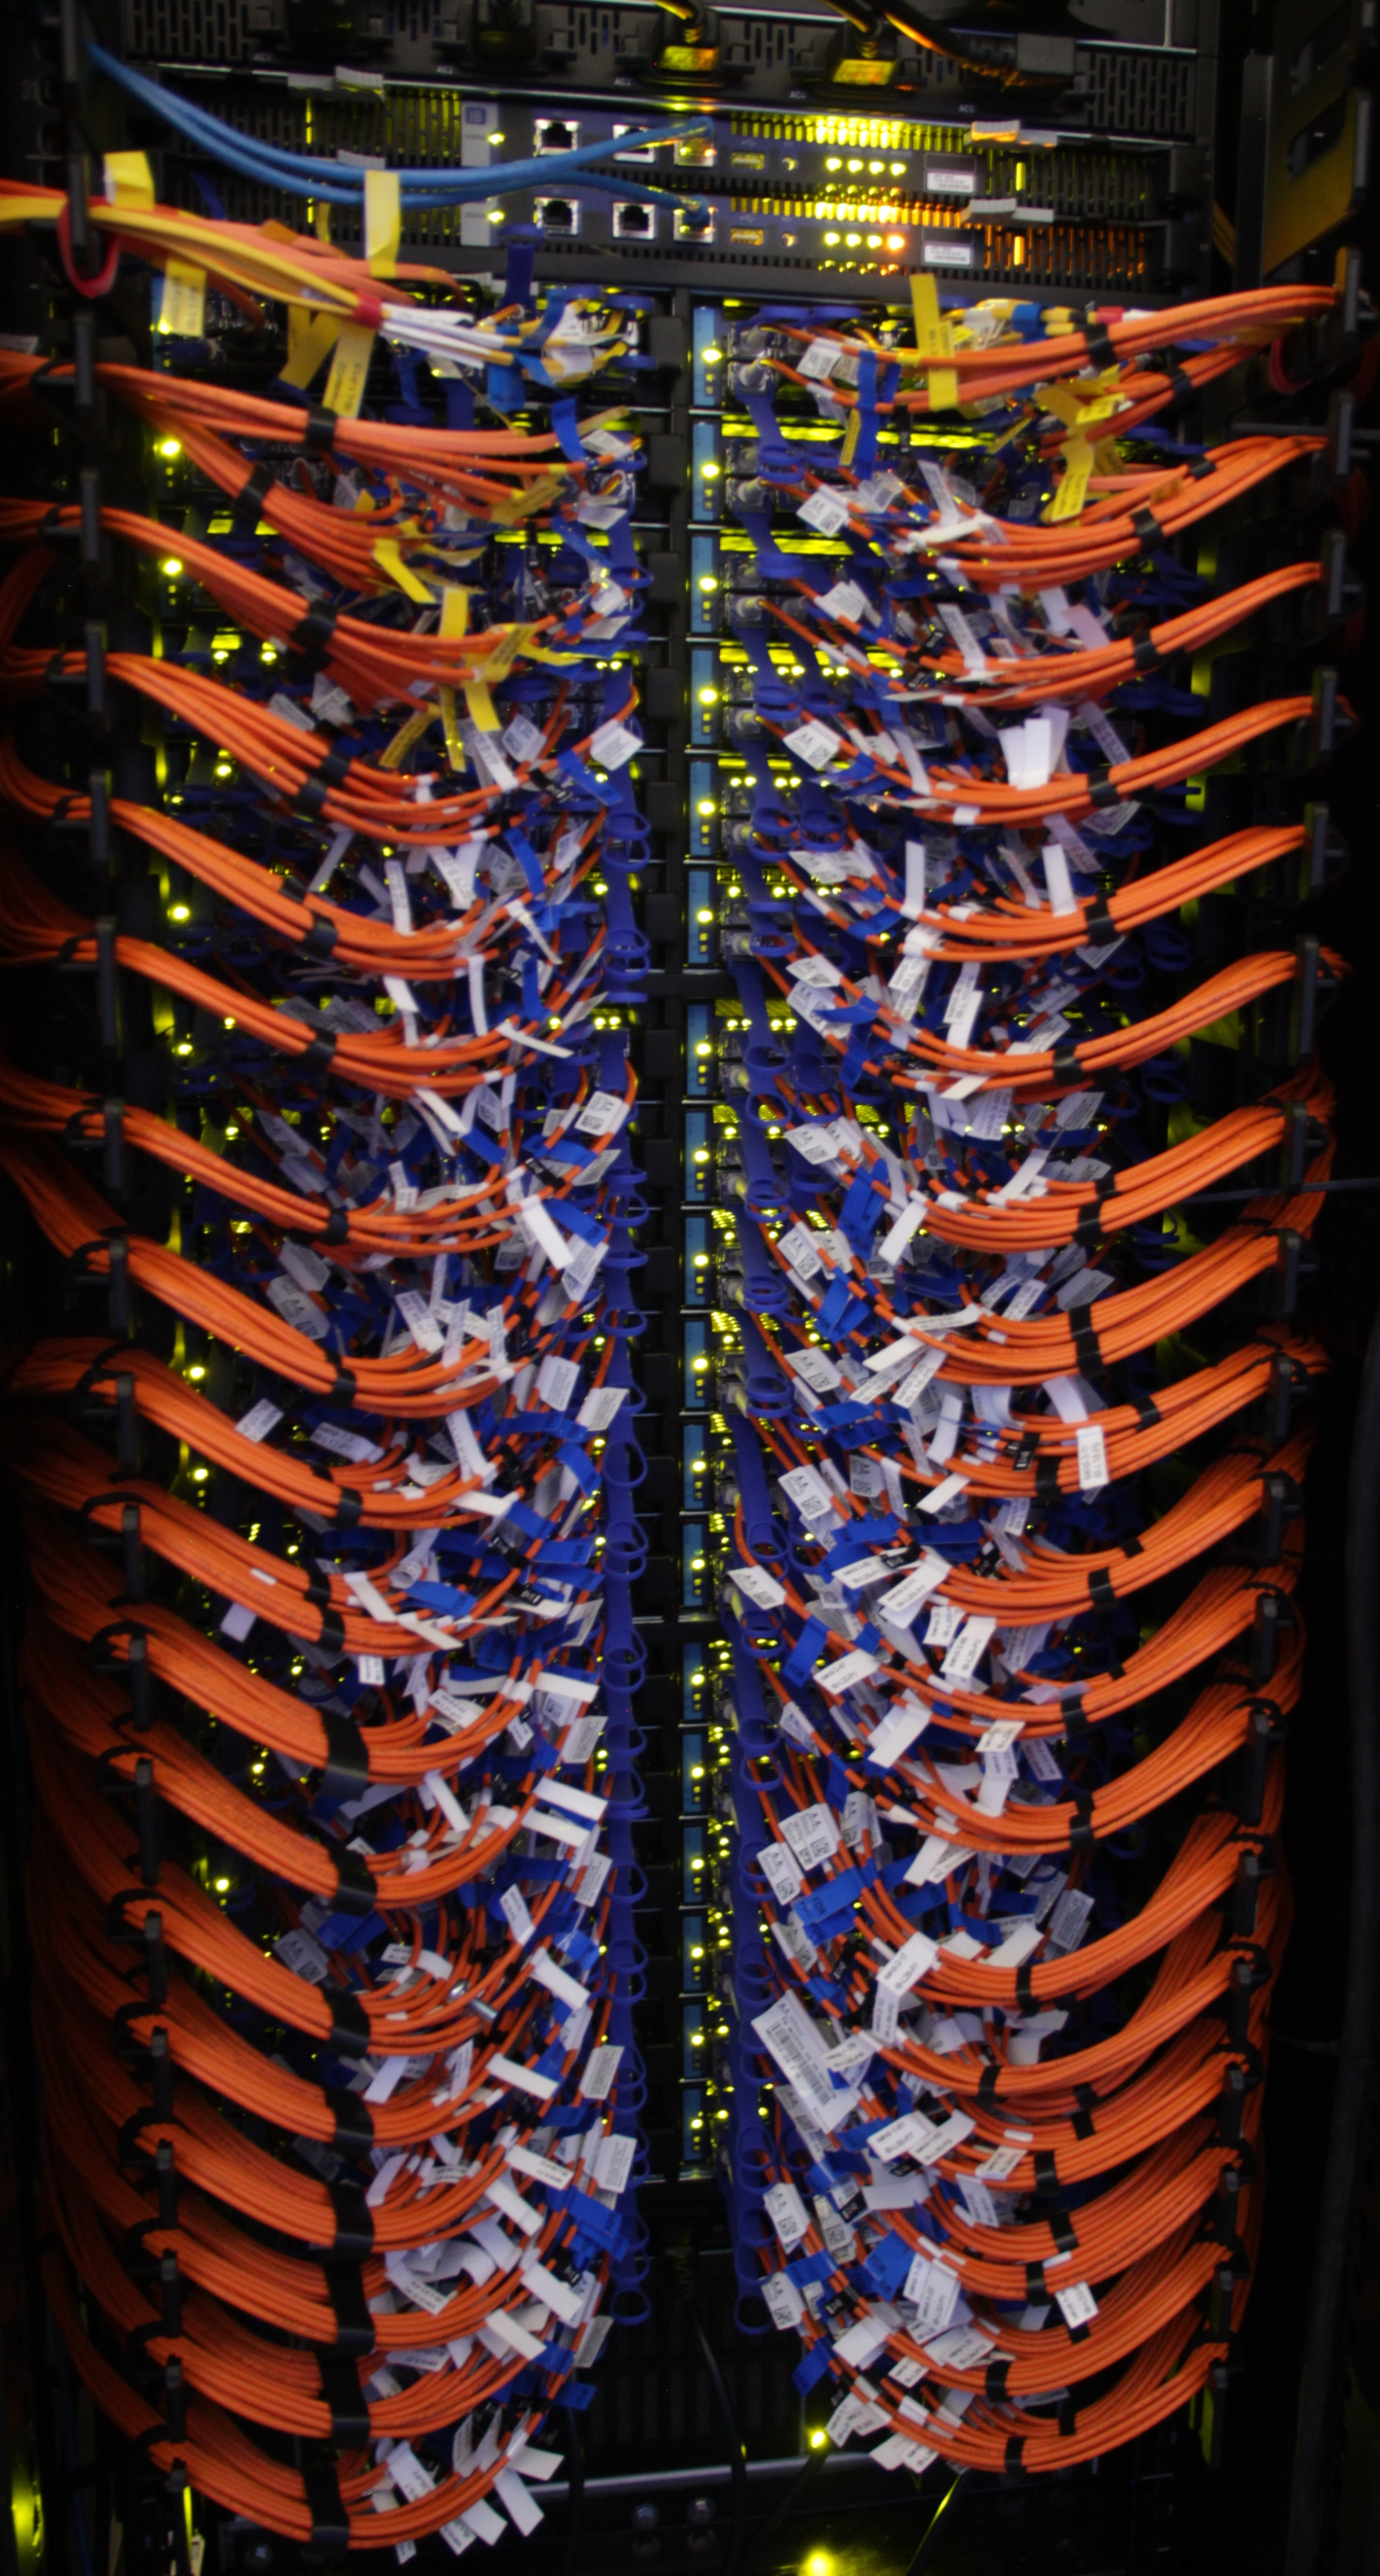
\includegraphics[height=0.85\textheight]{imgs/coreib.jpg}}\vss}\\
\end{tabular}
\end{frame}

% Choice: how tightly to couple the nodes - one big shared memory, or lots of distributed separate memories?
%pthreads, OpenMP
%MPI

\begin{frame}{Basics: How to Build a Supercomputer}
\begin{enumerate}
\setcounter{enumi}{2}
\item{Allocate CPUs \& memory to workload}
\begin{itemize}
\item{Clusters consist of distinct nodes (i.e. separate Linux computers), networked together and controlled centrally by a \alert{scheduler}.}
  \begin{itemize}
\pause
\item[$\ast$]{\alert{Each process/thread can see only its local node's CPUs and memory (without help from e.g. MPI).}}
\pause
\item[$\ast$]{\color{red}Each process/thread must fit within a single node's memory.}
\end{itemize}
\pause
\item{More expensive machines logically bind nodes into a single system.}
\begin{itemize}
\item[$\ast$]{Logically one big node.}
\item[$\ast$]{A single process can see the entire system.}
\item[$\ast$]{E.g.\ SGI UV.}
\end{itemize}
\end{itemize}
\end{enumerate}
\end{frame}

\section{Running Applications on a Cluster}
\begin{frame}{Basics: Running Applications on a Cluster}
\only<1-3>{\begin{itemize}
\item{Non-parallel (serial) code}
\begin{itemize}
\item[$\ast$]{\alert{For a single node as for a workstation.}}
\pause
\item[$\ast$]{Typically \alert{run as many copies per node as CPUs}, assuming node memory is sufficient.}
\pause
\item[$\ast$]{Or simply use the memory accompanying the remaining CPUs.}
\pause
\item[$\ast$]{\alert{Can replicate this across multiple nodes.}}
\end{itemize}
\end{itemize}}
\only<4->{\begin{itemize}
\item{Parallel code}
\begin{itemize}
\item<5->[$\ast$]{Thread parallelism works \alert{only within a node.}\hfill\\
E.g. pthreads, OpenMP.}
\item<6->[$\ast$]{MPI parallelism works \alert{both intra-{} and inter-node}.}
\item<7->[$\ast$]{Some \alert{hybrid} codes use both forms of parallel programming.}
\end{itemize}
\end{itemize}}
\end{frame}

%\section{Coprocessors}
%\begin{frame}{Basics: Coprocessors}{GPU computing}
%\end{frame}
%
%\section{Cluster Storage}
%\begin{frame}{Basics: Cluster Storage}{Data}
%\end{frame}
%
%\section{Resource Allocation}
%\begin{frame}{Basics: Resource Allocation}{Job scheduling}
%\end{frame}

\section{Summary}

\begin{frame}{Basics: Summary}

  % Keep the summary *very short*.
  \begin{itemize}
  \item<1->{\alert{Why have a supercomputer?}}
  \begin{itemize}\item<2->{Single problems requiring great time or big data; many problems.}\end{itemize}
  \item<3->{Most current supercomputers are \alert{clusters} of separate \alert{nodes}.}
  \item<4->{Each node has \alert{multiple CPUs} and \alert{(non-uniform, shared) memory}.}
  \item<5->{\alert{Parallel} code may use \alert{pthreads/OpenMP/MPI} within a node, or \alert{MPI} across multiple nodes.}
  \item<6->{\alert{Serial} code uses a single CPU and the memory of one node, but may be copied across many nodes.}
  \end{itemize}
  
\end{frame}

\part{Research Computing Services HPC}
\frame{\partpage}

%\begin{frame}{HPCS: Outline}
%\vskip -\bigskipamount
%\small\tableofcontents[subsectionstyle=hide]%[pausesections]
%  % You might wish to add the option [pausesections]
%\end{frame}

\section{Early History of Big Computers in Cambridge}

\begin{frame}<presentation>{Early History: EDSAC (1949--1958)}
\centerline{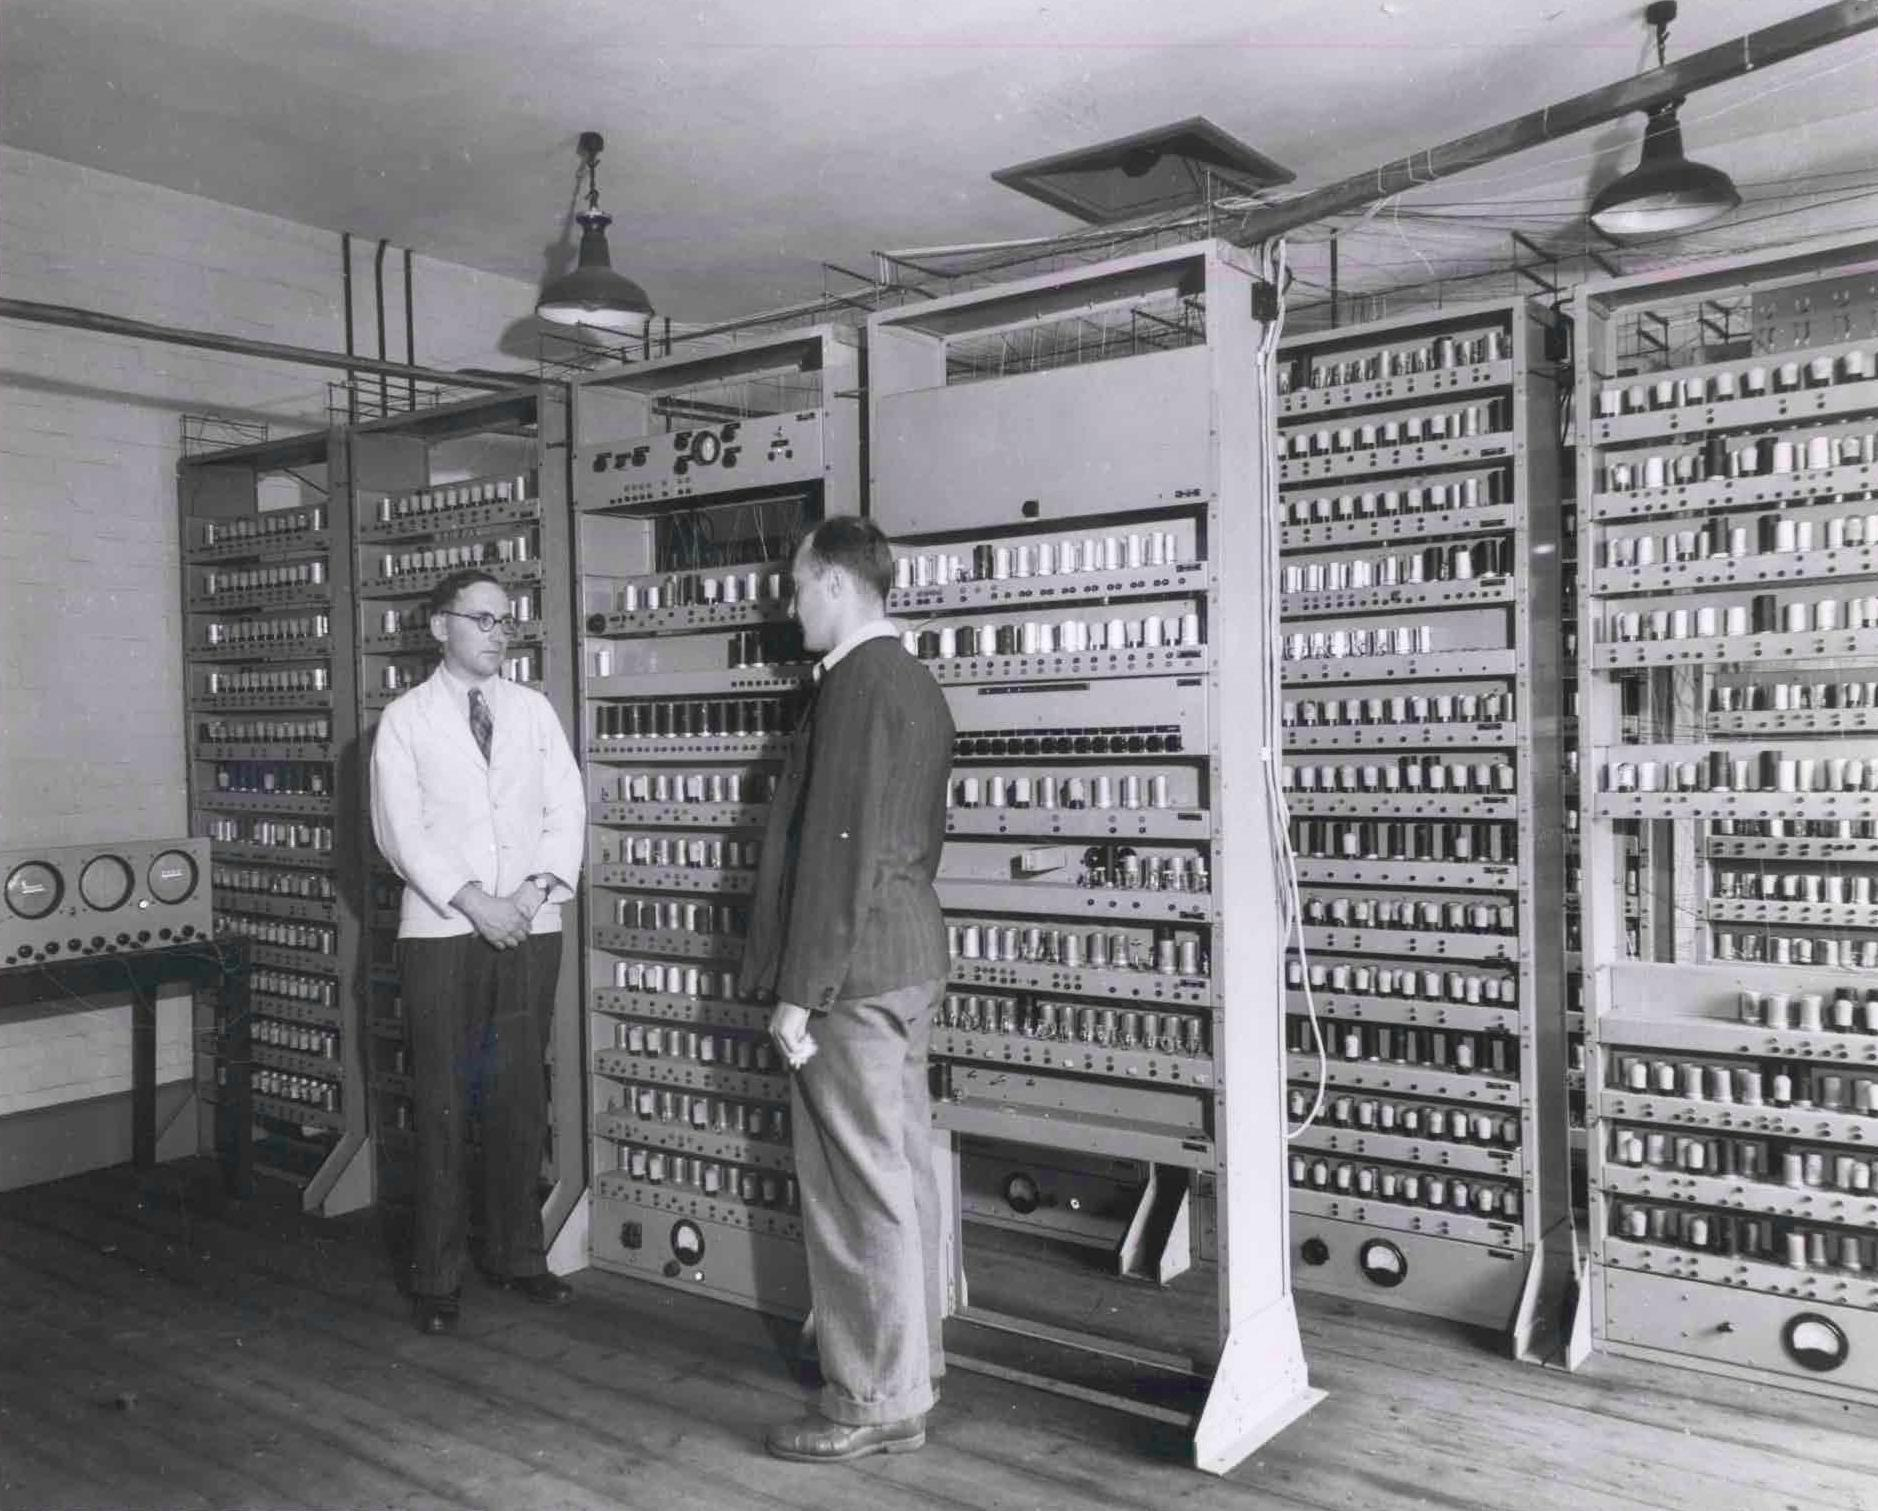
\includegraphics[width=0.8\textwidth]{imgs/edsac_wilkes.jpg}}%
\smallskip
\end{frame}

\begin{frame}{Early History: EDSAC (1949--1958)}
\begin{itemize}
\item{\textbf{E}lectronic \textbf{D}elay \textbf{S}torage \textbf{A}utomatic \textbf{C}alculator}
\item{The second general use, electronic digital (Turing complete) stored program computer}
\item{3,000 valves}
\item{650 instructions per second}
\item{2KB memory in mercury ultrasonic delay lines}
\item{One program at a time!}
\item{Used in meteorology, genetics, theoretical chemistry, numerical analysis, radioastronomy.}
\pause
\item{\emph{``On a few occasions it worked for more than 24 hours.''}}
\end{itemize}
\end{frame}

%\begin{frame}[fragile]{Early History: Mainframes (1958--1995)}
%\begin{description}
%\item[EDSAC 2 (1958--1965)]{{Complete redesign in-house: 10x faster, 80KB memory.}}
%\pause
%\item[TITAN (1964--1973)]{{Multiuser system, designed with Ferranti.}}
%\pause
% %\alert{\item[1970]{Mathematical Laboratory renamed as the Computer Laboratory and spins out the University Computing Service (UCS) to provide user services.}}
%%\pause
%\item[Phoenix (1971--1995)]{IBM mainframes, general purpose (including email).}
%\pause
%\alert{\item{Mainframe service morphs into distributed research computing support with central services.}}
%\pause
%\alert{\item{Specialised research computing needs remain!}}
%%\pause
%%\alert{\item{As does the pioneering tradition.}}
%\end{description}
%\end{frame}

\section{Central HPC in Cambridge}

\begin{frame}{Central HPC in Cambridge}
\begin{description}
\item[\alert{Created:}]{1996 (as the HPCF).}
\item[\alert{Mission:}]{Delivery and support of a large HPC resource for use by the University of Cambridge research community.}
\item<2->[\alert{Self-funding:}]{Paying and non-paying service levels.}
\item<2->[\alert{User base:}]{Includes external STFC \& EPSRC plus industrial users.}
\item<2->[\alert{Plus:}]{Dedicated group nodes and research projects.}
%\item<4->[\alert{2017}]{Research Computing Service (within the UIS).}
\end{description}
\end{frame}

\section{History of Performance}
\begin{frame}{History of Performance}
\rightline{http://www.top500.org}
\medskip
\begin{description}
\item[1997]{76.8 Gflop/s}
\item[2002]{1.4 Tflop/s}
\item[2006]{18.27 Tflop/s}
\item[2010]{30 Tflop/s}
\item[2012]{183.38 Tflop/s}
\item[2013]{$183.38\,\mbox{CPU}{}+ 239.90\,\mbox{GPU}$ Tflop/s}
\medskip
%\only<1>{\item[2017]{$1.697\,\mbox{CPU}{}+1.193\,\mbox{GPU}{}$ Pflop/s}}
\only<1->{\item[2018]{$\alert{2.271}\,\mbox{CPU}{}+1.193\,\mbox{GPU}{}$ Pflop/s}}
\end{description}
\end{frame}

\begin{frame}<presentation>{Darwin1 (2006--2012)}
\centerline{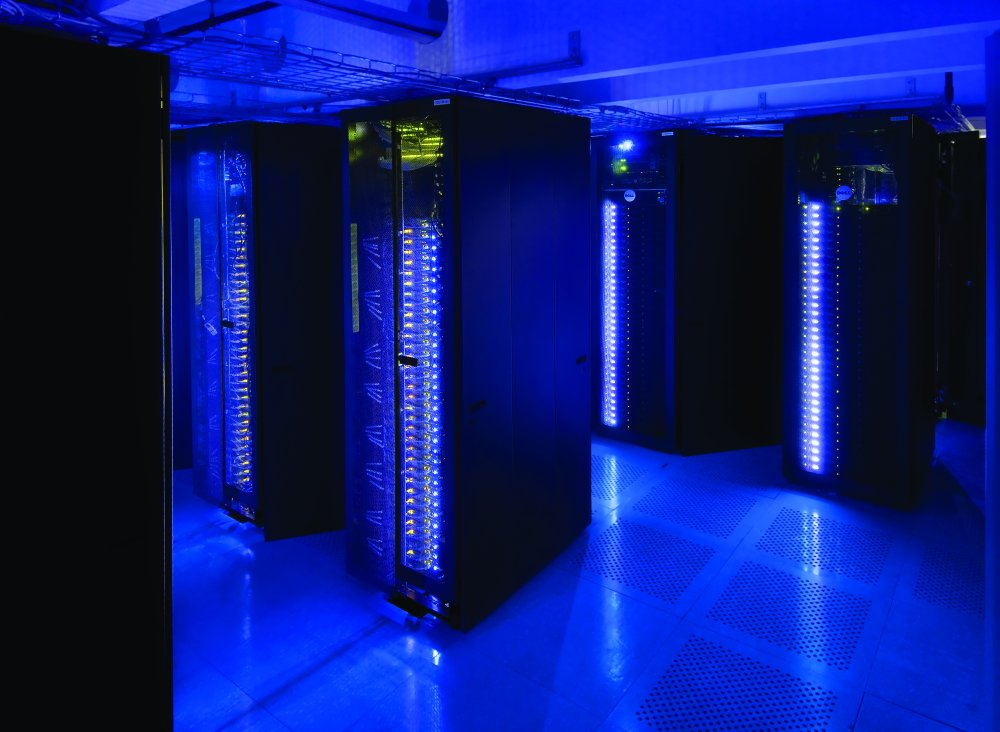
\includegraphics[width=0.875\textwidth]{imgs/darwin.jpg}}%
\smallskip
\end{frame}

\begin{frame}<presentation>{Darwin3 (2012--2018)(b) \& Wilkes (2013--2018)(f)}
\only<1>{\centerline{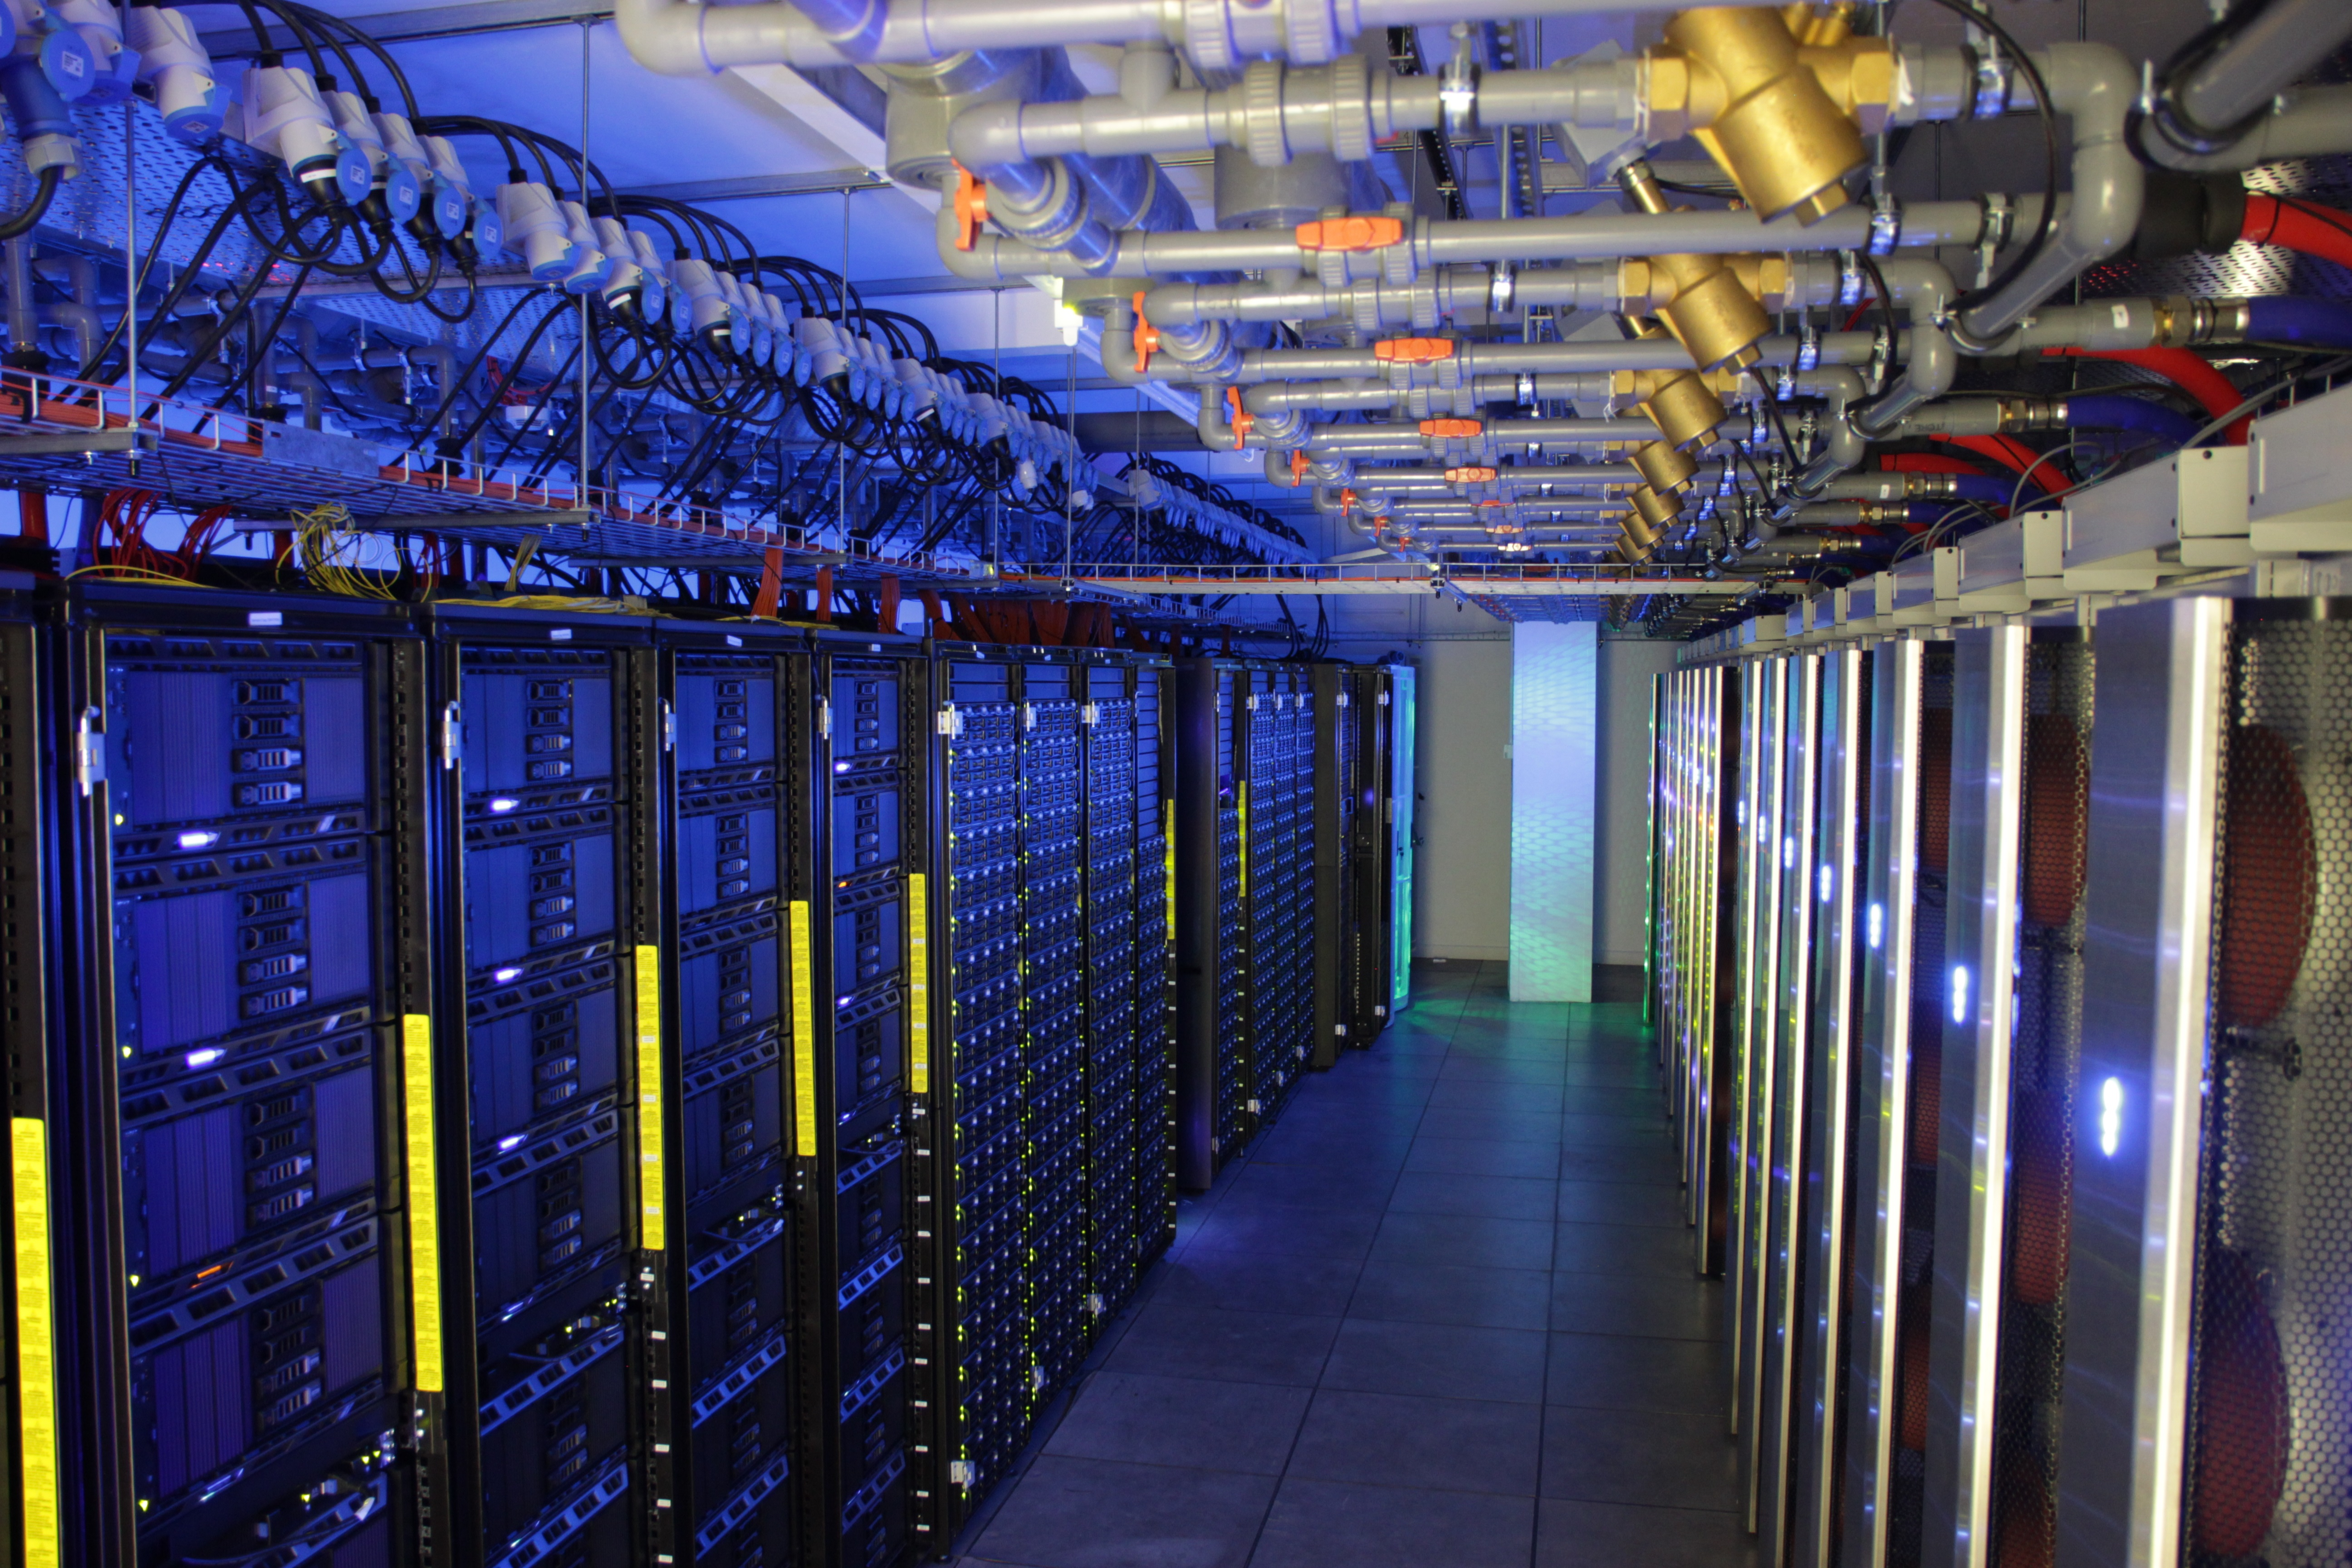
\includegraphics[width=0.95\textwidth]{imgs/MLDC-big.jpg}}}%
%\only<2>{\centerline{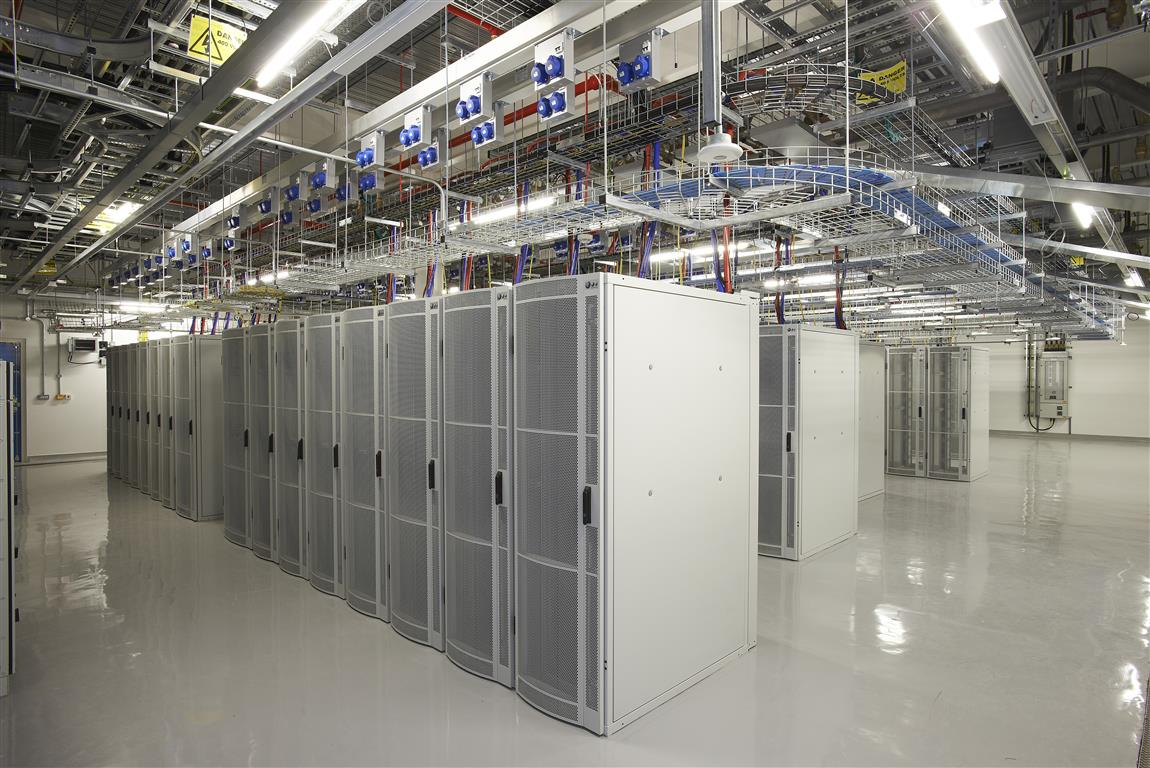
\includegraphics[width=0.95\textwidth]{imgs/WCDC-HPCS.jpg}}}%
\smallskip
\end{frame}

\begin{frame}<presentation>{Peta4 (2017) Cumulus (2018)}
\only<1>{\centerline{
\includegraphics[width=0.95\textwidth]{imgs/peta4.jpg}}}%
\smallskip
\end{frame}


%\section{CSD3}
%\begin{frame}{CSD3 - University of Cambridge}
%\begin{itemize}
%\item{Cambridge Service for Data Driven Discovery}
%\pause
%\medskip
%\item{\alert{Peta4 --- Intel CPU cluster}}
%\pause
%\item{\alert{Wilkes2 --- NVIDIA GPU cluster}}
%\pause
%\medskip
%\item{Hadoop-based data analytic platform}
%\item{Burst buffer}
%\end{itemize}
%\end{frame}

\section{Skylake}
\begin{frame}{Skylake}
\begin{itemize}
\item{Each compute node:}
\begin{itemize}
\item[$\ast$]{\only<1>{2x16 cores, Intel Skylake 2.6 GHz}\only<2->{{\color{red}32 CPUs}}}
\item[$\ast$]{\only<1>{$192\,\text{GB}$ or $384\,\text{GB}$ RAM}\only<2->{{\color{red}$6\,\text{GB}$ or $12\,\text{GB}$ per CPU}}}
\item[$\ast$]{\only<1>{$100\,\text{Gb/sec}$ Omni-Path}\only<2->{\color{red}$10\,\text{GB/sec}$ (for MPI and storage)}}
\end{itemize}
\item{1152 compute nodes.}
\item{8 login nodes (\alert{login-cpu.hpc.cam.ac.uk}).}
\end{itemize}
\end{frame}

\section{Coprocessors --- GPUs etc}
\begin{frame}{Coprocessors --- GPUs etc}
  \begin{itemize}
  \item{CPUs are \alert{general purpose}}
    \pause
  \item{Some types of parallel workload fit \alert{vector} processing well:}
    \begin{itemize}
    \item{Single Instruction, Multiple Data (SIMD)}
    \item{\emph{Think pixels on a screen}}\pause
    \item{GPUs specialise in this type of work}\pause
      \item{Also competitor many-core architectures such as the Intel Phi}
    \end{itemize}
\end{itemize}
\end{frame}

\section{Pascal}
\begin{frame}{Pascal}
\begin{itemize}
\item{Each compute node:}
\begin{itemize}
\item[$\ast$]{\only<1>{$4\times\text{NVIDIA P100 GPU}$}\only<2->{\color<2->{red}4 GPUs}}
\item[$\ast$]{\only<1>{1x12 cores, Intel Broadwell 2.2 GHz}\only<2->{{\color{red}12 CPUs}}}
\item[$\ast$]{\only<1>{$96\,\text{GB}$ RAM}\only<2->{{\color{red}$96\,\text{GB}$ RAM}}}
\item[$\ast$]{\only<1>{$100\,\text{Gb/sec}$ (4X EDR) Infiniband.}\only<2->{\color{red}$10\,\text{GB/sec}$ (for MPI and storage)}}
\end{itemize}
\item{90 compute nodes.}
\item{8 login nodes (\alert{login-gpu.hpc.cam.ac.uk}).}
\end{itemize}
\end{frame}

\section{KNL}
\begin{frame}{KNL (Intel Phi)}
\begin{itemize}
\item{Each compute node:}
\begin{itemize}
\item[$\ast$]{\only<1>{64 cores, Intel Phi 7210}\only<2->{{\color{red}256 CPUs}}}
\item[$\ast$]{\only<1>{$96\,\text{GB}$ RAM}\only<2->{{\color{red}$96\,\text{GB}$ RAM}}}
\item[$\ast$]{\only<1>{$100\,\text{Gb/sec}$ Omni-Path}\only<2->{\color{red}$10\,\text{GB/sec}$ (for MPI and storage)}}
\end{itemize}
\item{342 compute nodes}
\item{Shared login nodes with Skylake}
\end{itemize}
\end{frame}


%\begin{frame}{HPCS Production Cluster Schematic}
%\centerline{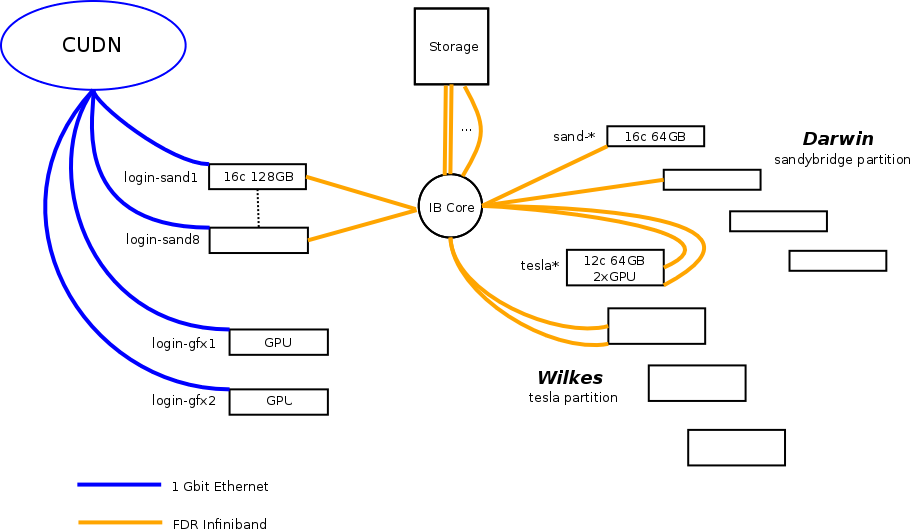
\includegraphics[width=0.95\textwidth]{imgs/cluster.png}}%
%\end{frame}

\section{Storage}
\begin{frame}{Cluster Storage}
  \begin{itemize}
\item{Lustre cluster filesystem:}
  \begin{itemize}
\item[$\ast$]{Very scalable, high bandwidth.}
\item[$\ast$]{Multiple RAID6 back-end disk volumes.}
\item[$\ast$]{Multiple object storage servers.}
\item[$\ast$]{Single metadata server.}
\item[$\ast$]{Tape-backed HSM on newest filesystems.}
\item[$\ast$]{\alert{$12\,\text{GB/sec}$ overall read or write.}}
\item[$\ast$]{\alert{Prefers big read/writes over small.}}
\end{itemize}
\end{itemize}
\end{frame}

\section{Obtaining an Account and Support}
\begin{frame}{Obtaining an Account and Support}
\begin{itemize}
\item{\alert{https://www.hpc.cam.ac.uk/applications-access-research-computing-services}}
\item{Email \alert{support@hpc.cam.ac.uk}}
\end{itemize}
\end{frame}

\part{Using HPC}
\frame{\partpage}

\section{Connecting}
\begin{frame}{Using HPC: Connecting to the RCS Clusters}
\begin{itemize}
\item SSH secure protocol only.\hfill\\
\visible<2->{\alert{Supports login, file transfer, remote desktop\ldots}}
\item<3-> SSH access is allowed from anywhere.\hfill\\
\visible<4->{\alert{Fail2Ban will ban repeatedly failing clients for 20 minutes.}}\hfill\\
%\visible<5->{\alert{This is a change compared to the earlier clusters.}}
\item<5->{Policies for other clusters may differ.}
\end{itemize}
\end{frame}

\subsection{Windows Clients}
\begin{frame}{Connecting: Windows Clients}
\begin{itemize}
\item<1-5> putty, pscp, psftp\hfill\\
\alert{\small http://www.chiark.greenend.org.uk/~sgtatham/putty/download.html}
\item<2-5> WinSCP\hfill\\
\alert{\small http://winscp.net/eng/download.php}
\item<3-5> TurboVNC \alert{\small (remote desktop, 3D optional)}\hfill\\
\alert{\small http://sourceforge.net/projects/turbovnc/files/}
\item<4-5> Cygwin \visible<4->{\alert{\small (provides an application environment similar to Linux)}}\hfill\\
\alert{\small http://cygwin.com/install.html}\hfill\\
\visible<5>{\alert{\small Includes X server for displaying graphical applications running remotely.}}
\item<6> MobaXterm\hfill\\
\alert{\small http://mobaxterm.mobatek.net/}
\end{itemize}
\end{frame}

\subsection{Linux/MacOSX/UNIX Clients}
\begin{frame}{Connecting: Linux/MacOSX/UNIX Clients}
\begin{itemize}
\item {\color<2->{red}ssh}, scp, sftp, {\color<2->{red}rsync}\hfill\\
\alert{\small Installed (or installable).}
\item<3-> TurboVNC \alert{\small (remote desktop, 3D optional)}\hfill\\
\alert{\small http://sourceforge.net/projects/turbovnc/files/}
\item<4-> On MacOSX, install \alert{XQuartz} to display remote graphical applications.\hfill\\
\alert{\small http://xquartz.macosforge.org/landing/}
\end{itemize}
\end{frame}

\subsection{Login}
\begin{frame}{Connecting: Login}
\begin{itemize}
\item From Linux/MacOSX/UNIX (or Cygwin):\hfill\\
\alert{ssh -Y \textbf{abc123}@login-cpu.hpc.cam.ac.uk}
\pause
\item From graphical clients:\hfill\\
Host: \alert{login-cpu.hpc.cam.ac.uk}\hfill\\
Username: \alert{\textbf{abc123}} (your UCAM account name)
\pause
\item login-cpu.hpc will map to a random login node\hfill\\
\alert{i.e. one of login-e-9, login-e-10,\,\ldots\,, login-e-16}
\end{itemize}
\end{frame}

\subsection{First time login}
\begin{frame}{Connecting: First time login}
\begin{itemize}
\item{The first connection to a particular hostname produces the following:}
\begin{semiverbatim}\tiny
  The authenticity of host 'login-cpu (128.232.224.50)' can't be established.

  
  {\color<2->{red}ECDSA key fingerprint is SHA256:HsiY1Oe0M8tS6JwR76PeQQA/VB7r8675BzG5OYQ4h34.}
  
  {\color<2->{red}ECDSA key fingerprint is MD5:34:9b:f2:d2:c6:b3:5c:63:99:b7:27:da:5b:c8:16:fe.}
  

  Are you sure you want to continue connecting (yes/no)? {\color<3->{red}yes}

Warning: Permanently added 'login-cpu,128.232.224.50' (ECDSA) to the list of known hosts.
 \end{semiverbatim}
\smallskip\item{\alert{One should always check the fingerprint before typing ``yes''.}}
\item{Graphical SSH clients \emph{should} ask a similar question.}
\item{Designed to detect fraudulent servers.}
\end{itemize}
\end{frame}

\begin{frame}[fragile]{Connecting: First time login}
\begin{itemize}
\item{Exercise 1 - Log into your RCS training account.}
  \pause
  \item{Exercise 2 - Simple command line operations.}
\end{itemize}
\end{frame}

\subsection{File Transfer}
\begin{frame}{Connecting: File Transfer}
\begin{itemize}
\item With graphical clients, connect as before and drag and drop.
\pause
\item From Linux/MacOSX/UNIX (or Cygwin):\hfill\\
\alert{\footnotesize rsync -av \textbf{old\_directory/} abc12@login-cpu.hpc.cam.ac.uk:rds/hpc-work/new\_directory}\hfill\\
copies contents of old\_directory to $\tilde{}\text{/rds/hpc-work/new\_directory}$.\hfill\\\smallskip
\pause
\alert{\footnotesize rsync -av \textbf{old\_directory} abc12@login-cpu.hpc.cam.ac.uk:rds/hpc-work/new\_directory}\hfill\\
copies old\_directory (and contents) to $\tilde{}\text{/rds/hpc-work/new\_directory/old\_directory}$.\hfill\\
\pause
\begin{itemize}
\item[$\ast$]Rerun to update or resume after interruption.
\item[$\ast$]All transfers are checksummed.
\item[$\ast$]For transfers in the opposite direction, place the remote machine as the first argument.
\end{itemize}
\pause
\item{Exercise 3 - File transfer.}
\end{itemize}
\end{frame}

\subsection{Remote Desktop}
\begin{frame}[fragile]{Connecting: Remote Desktop}
\begin{itemize}
\item First time use of TurboVNC (recommended):
\begin{semiverbatim}
\footnotesize
[sjr20@login-e-1 ~]\$ vncserver

You will require a password to access your desktops.

Password: 
Verify:   
Would you like to enter a view-only password (y/n)? n

New 'login-e-1:99 (sjr20)' desktop is {\color{red}login-e-1:99}

Starting applications specified in /home/sjr20/.vnc/xstartup
Log file is /home/sjr20/.vnc/login-e-1:99.log
\end{semiverbatim}
\item{NB Choose a \alert{different} password for VNC to protect your desktop from other users.}
\item{Note the unique host and display number ({\color{red}login-e-1} and {\color{red}:99} here).}
\end{itemize}
\end{frame}

\begin{frame}[fragile]{Connecting: Remote Desktop}
\begin{itemize}
\item Remote desktop already running:
\begin{semiverbatim}
\footnotesize
[sjr20@login-e-1 ~]\$ vncserver -list

TigerVNC server sessions:

X DISPLAY #     PROCESS ID
:99             130655
\end{semiverbatim}
\smallskip\item Kill it:
\begin{semiverbatim}
\footnotesize
[sjr20@login-e-1 ~]\$ vncserver -kill :99
Killing Xvnc process ID 130655
\end{semiverbatim}
\smallskip\item\alert{Typically you only need {\color{red}one} remote desktop.}
\item\alert{Keeps running until killed, or the node reboots.}
\end{itemize}
\end{frame}

\begin{frame}[fragile]{Connecting: Remote Desktop}
\begin{itemize}
\item To connect to the desktop from Linux:\\\hfill\break
{\scriptsize
\alert{vncviewer -via abc12@login-e-1.hpc.cam.ac.uk localhost:99}}
\smallskip
\item{The display number \alert{:99} will be different in general and unique to each desktop.}
\item{You will be asked firstly for your cluster login password, and secondly for your VNC password.}
\item{\alert{Press F8 to bring up the control panel.}}
\pause
\item{Exercise 4 - Connecting to a remote desktop running on the HPC cluster.}
\end{itemize}
\end{frame}


%\begin{frame}{TurboVNC Session}
%\begin{center}
%\centerline{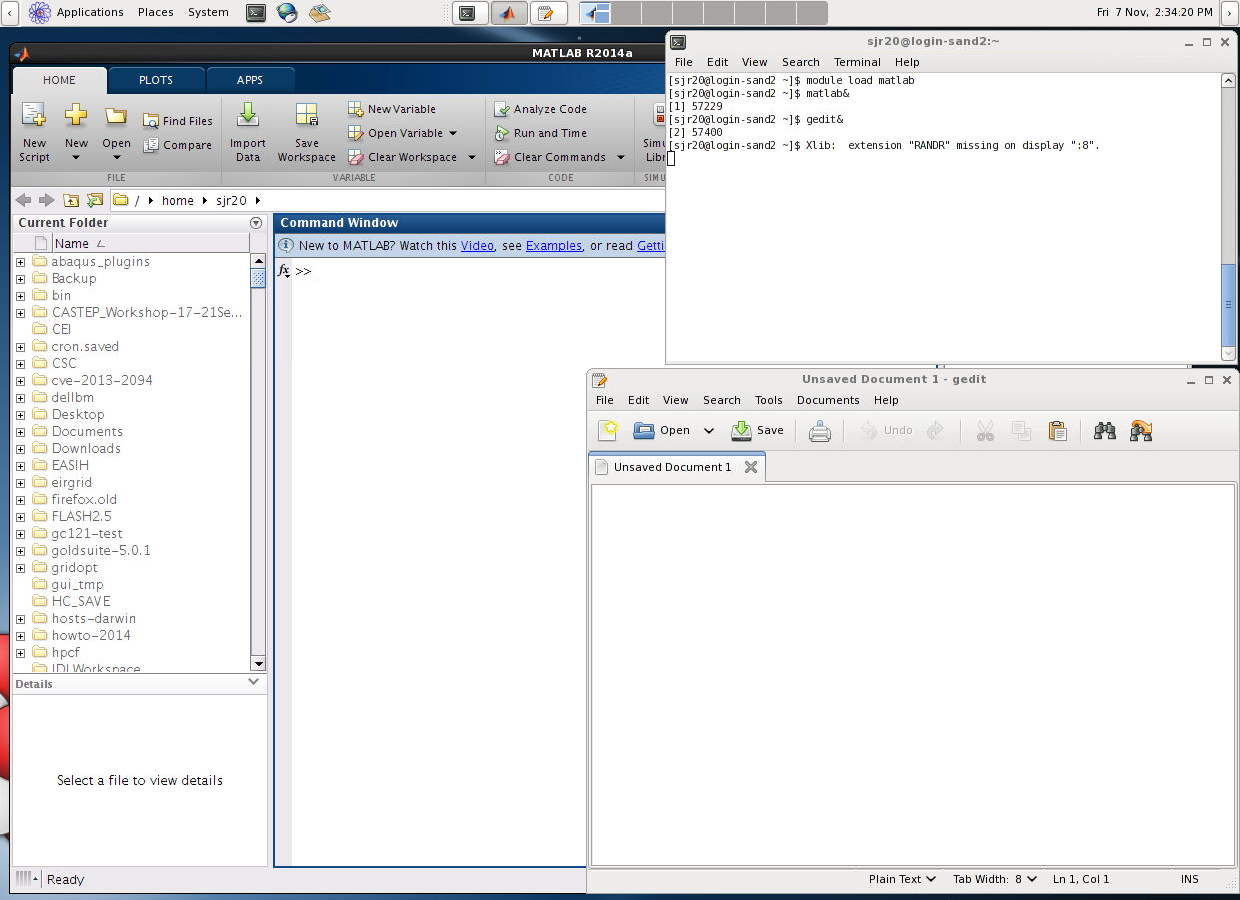
\includegraphics[width=0.85\textwidth]{imgs/linux-turbovnc.png}}
%\end{center}
%\end{frame}

%\begin{frame}{Linux TurboVNC Control Panel}
%\begin{center}
%\centerline{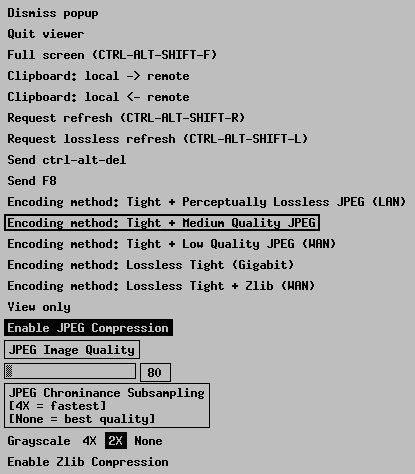
\includegraphics[height=0.8\textheight]{imgs/linux-turbovnc-F8.png}}
%\end{center}
%\end{frame}

%\begin{frame}{Connecting: Remote Desktop (MobaXterm)}
%\begin{center}
%\centerline{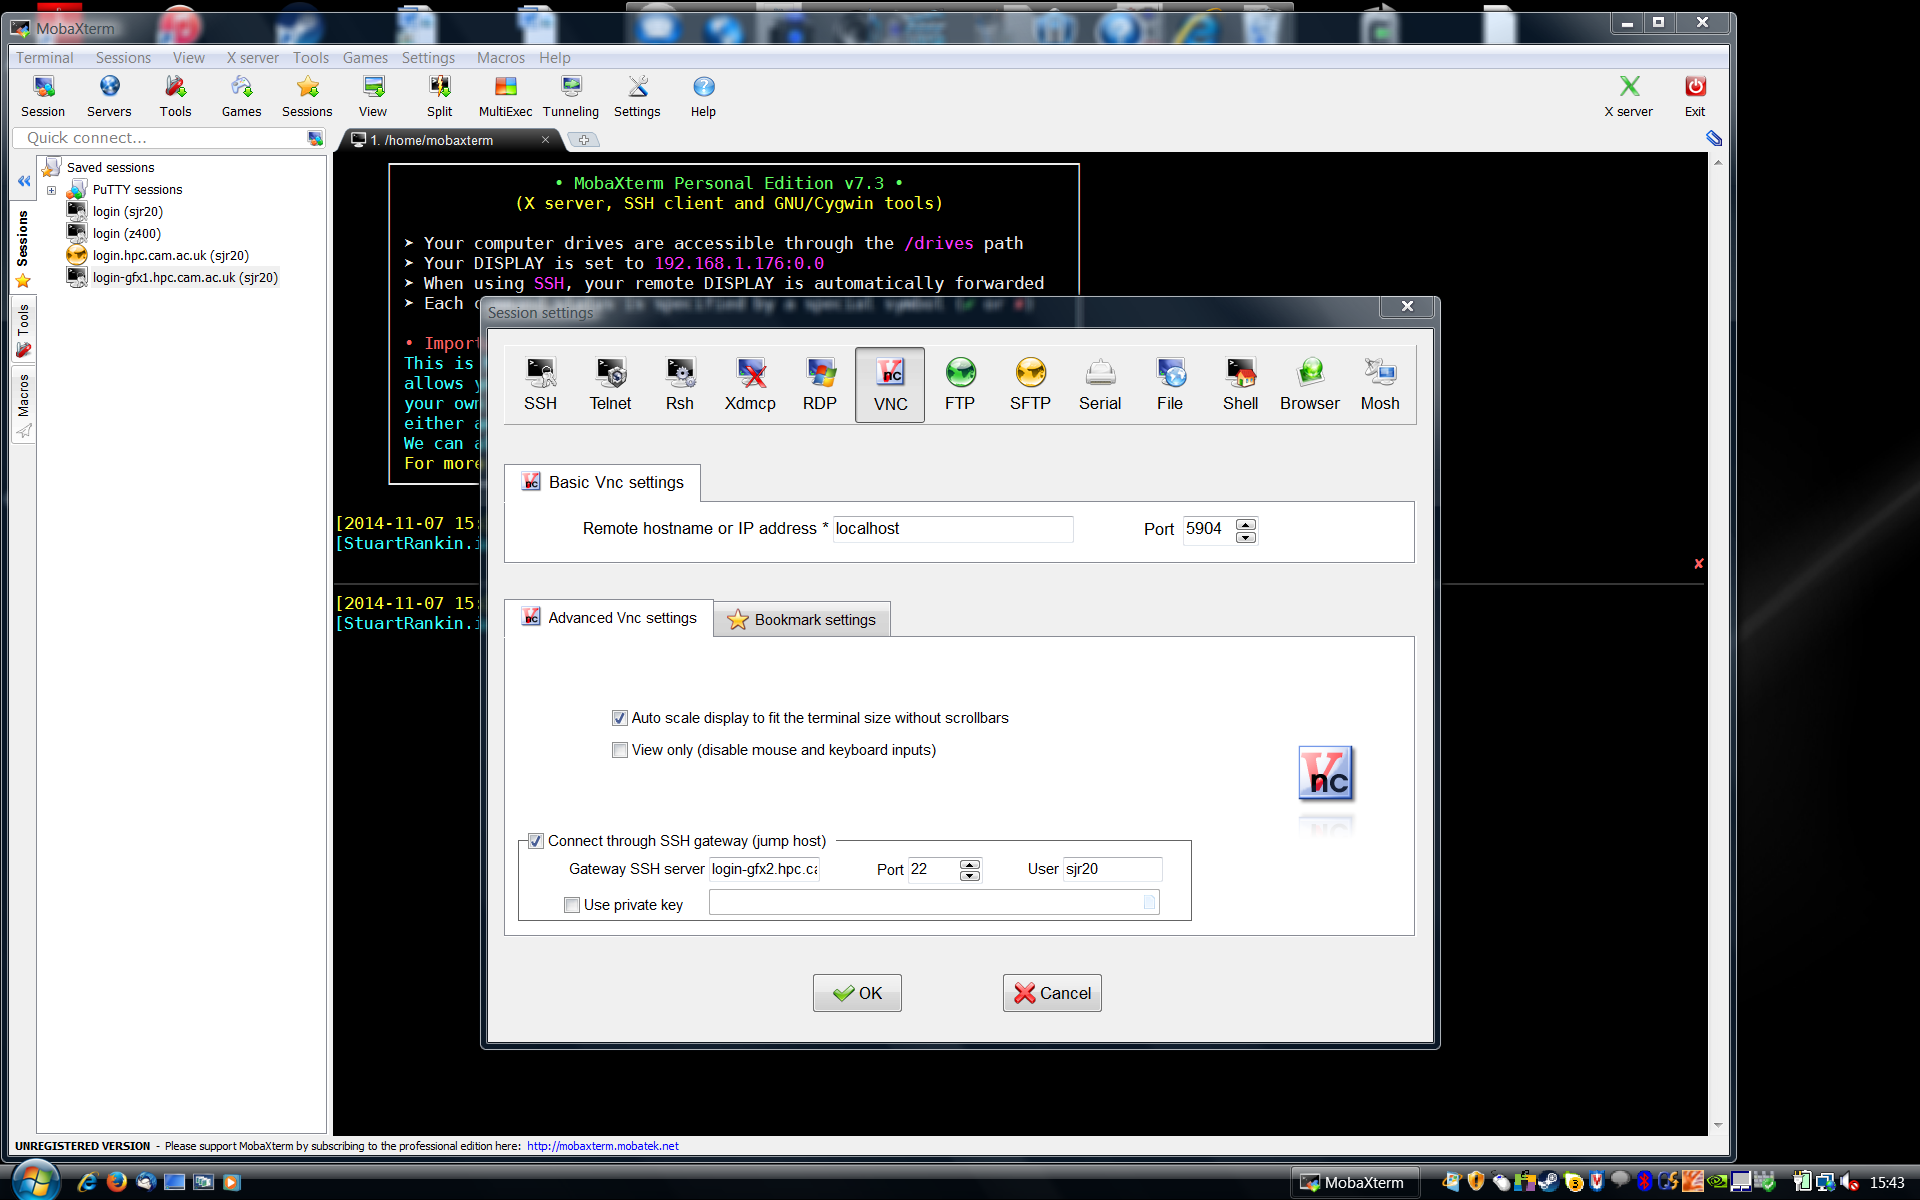
\includegraphics[height=0.8\textheight]{imgs/mobaxterm-turbovnc.png}}
%\end{center}
%\end{frame}

%\begin{frame}{Connecting: Remote Desktop (MobaXterm)}
%\begin{center}
%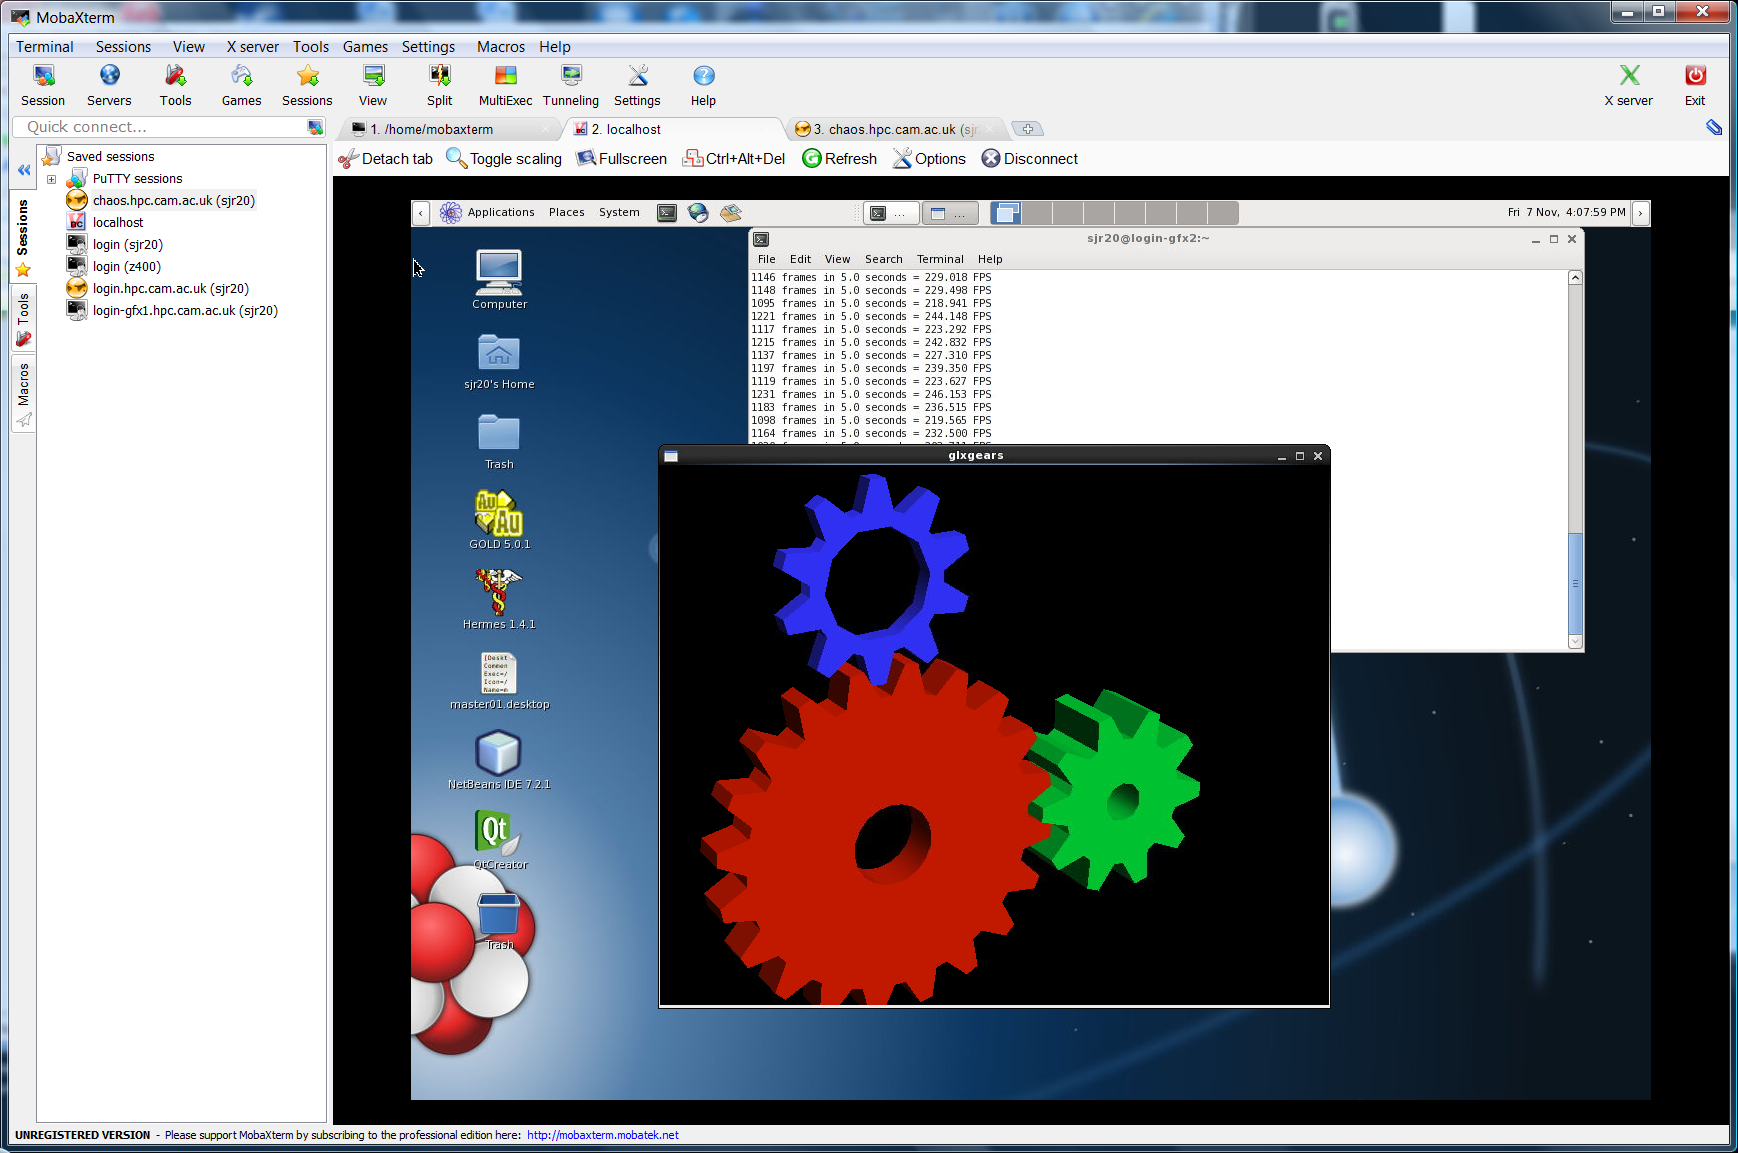
\includegraphics[height=0.8\textheight]{imgs/mobaxterm-vgl-turbovnc.png}
%\end{center}
%\end{frame}

%\begin{frame}{3D Remote Visualization}
%\begin{center}
%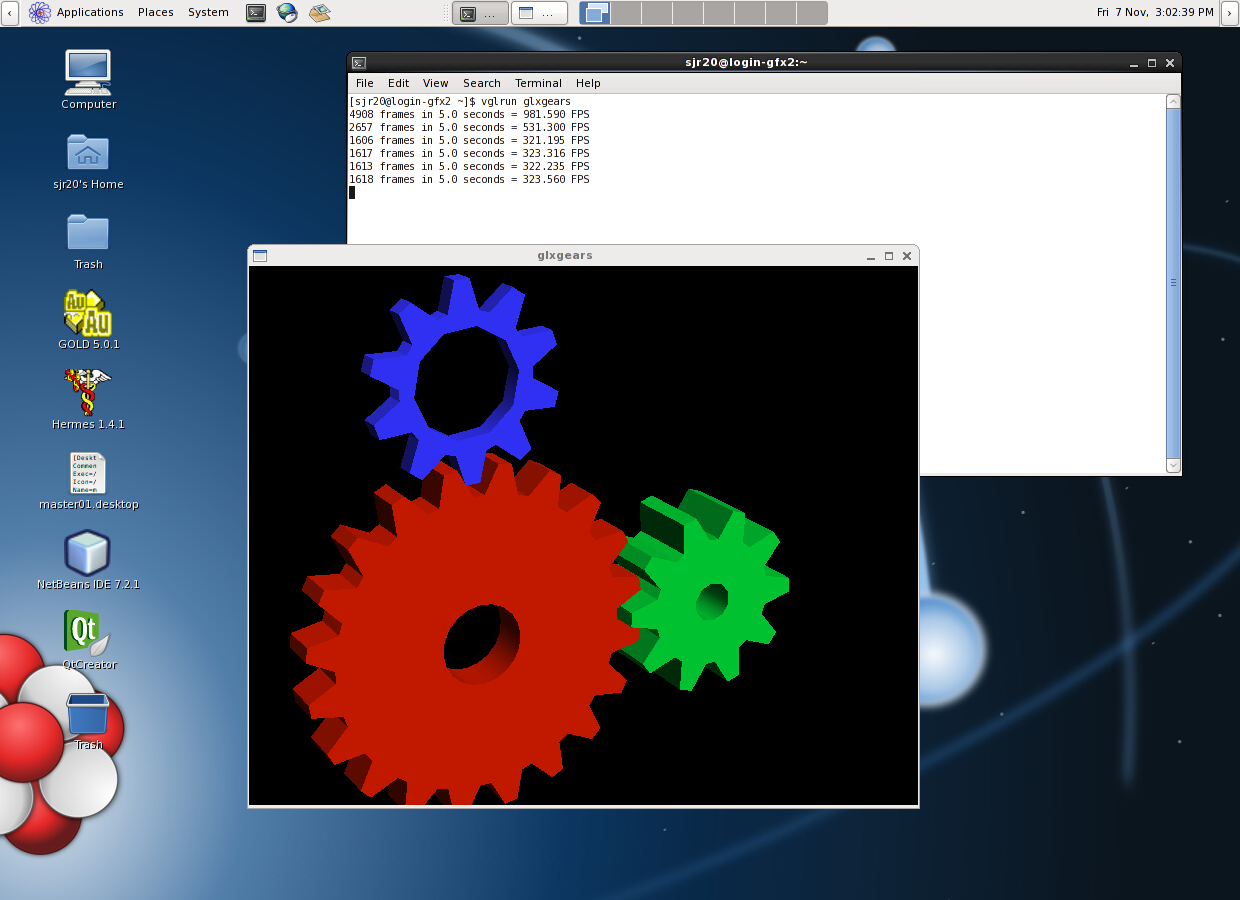
\includegraphics[height=0.8\textheight]{imgs/vgl-turbovnc.png}
%\end{center}
%\end{frame}


%12:00
%Lunch
%14:00

\section{User Environment}
\begin{frame}{Using HPC: User Environment}
\begin{itemize}
\item<1,3->{\visible<1>{Scientific Linux 7.x (}\alert<1>{{\color<3->{red}Red Hat Enterprise Linux 7}\visible<1>{.x rebuild)}}}
\begin{itemize}
\item{\visible<1>{bash shell}}
\item{\visible<1>{Gnome or XFCE4 desktop \alert{(if you want)}}}
\item{\visible<1>{GCC, Intel, PGI compilers and other development software.}}
\end{itemize}
\item<2->{But you don't need to know that.}
\item<4->{\color{red}NOT Ubuntu or Debian!}
\item<5>{\alert{CentOS 7 is OK.}}
\end{itemize}
\end{frame}

\subsection{Filesystems}
\begin{frame}{User Environment: Filesystems}
\begin{itemize}
\item{\alert{/home/abc123}}
\begin{itemize}
\item{40GB quota.}
\item{Visible equally from all nodes.}
\item{Single storage server.}
\item{Hourly, daily, weekly snapshots copied to tape.}
\item{Not intended for job outputs or large/many input files.}
\end{itemize}
\item{\alert{/rds/user/abc123/hpc-work} a.k.a.\ \alert{/home/abc123/rds/hpc-work}}
\begin{itemize}
\item{Visible equally from all nodes.}
\item{Larger and faster (1TB initial quota).}
\item{Intended for job inputs and outputs.}
\item{{\color{red}Not backed up.}}
  \pause
  \item{\alert{Research Data Storage}}
  \item{\alert{https://www.hpc.cam.ac.uk/research-data-storage-services}}
\end{itemize}
\end{itemize}
\end{frame}

\begin{frame}[fragile]{Filesystems: Quotas}
\begin{itemize}
\item{quota}
\begin{semiverbatim}
\tiny
[abc123@login-e-1 ~]$ quota
Filesystem  GiBytes    quota   limit   grace    files    quota    limit   grace User/group
/home          10.6     40.0    40.0       0    ----- No ZFS File Quotas  ----- U:abc123
/rds-d2         1.0   1024.0  1126.4       -        8  1048576  1048576       - G:abc123
\end{semiverbatim}
\item<1-|handout:1->{\alert{Aim to stay below the soft limit (\emph{quota}).}}
\item<2-|handout:1->{\alert{Once over the soft limit, you have 7 days grace to return below.}}
\item<3-|handout:2>{\alert{When the grace period expires, or you reach the hard limit (\emph{limit}), no more data can be written.}}
\item<4-|handout:2>{\alert{It is important to rectify an out of quota condition ASAP.}}
\end{itemize}
\end{frame}

%\begin{frame}{Filesystems: Backups???}
%\begin{itemize}
%\item<1->{Disk snapshots and tape (as of May 2017).}
%\item<2->{{\color{red}They are not an undelete - take care when deleting.}}
%\item<3->{Successful restoration depends on:}
%\begin{itemize}
%\item{The file having existed long enough to have been backed up at all.}
%\item{The last good version existing in a current backup.}
%\item<4->{\color{red}Request restoration as soon as possible with \emph{location} and \emph{exact time of loss}.}
%\medskip
%\visible<5->{\item{\color{purple}\huge Scratch files are not backed up.}}
%\end{itemize}
%\end{itemize}
%\end{frame}

%\begin{frame}{Filesystems: Automounter}
%\begin{itemize}
%\item{Directories under /rds/user and /rds/project are \alert{automounted}.}
%\item{They only appear when explicitly referenced.}
%\item{Thus when browsing these directories may appear too empty\hfill\\
%  \qquad\alert{--- use \emph{ls} or \emph{cd} to reference /rds/user/abc123 explicitly.}}
%  \item{We create convenience symlinks (shortcuts) under \~{}/rds.}
%\end{itemize}
%\end{frame}

\begin{frame}{Filesystems: Permissions}
\begin{itemize}
\item{\color{red}Be careful and if unsure, please ask support.}
\begin{itemize}
\item{Can lead to \alert{accidental destruction} of your data or \alert{account compromise}.}
\end{itemize}
\item{Avoid changing the permissions on your home directory.}
\begin{itemize}
\item{Files under /home are particularly security sensitive.}
\item{Easy to break passwordless communication between nodes.}
\end{itemize}
\end{itemize}
\end{frame}

\subsection{Software}
\begin{frame}{User Environment: Software}
\begin{itemize}
\item{Free software accompanying \alert{Red Hat Enterprise Linux} is (or can be) provided.}
\item{Other software (free and non-free) is available via \alert{modules}.}
\item{Some proprietary software may not be generally accessible.}
\item{New software may be possible to provide on request.}
\item{\alert{Self-installed software should be properly licensed.}}
  \pause
\item{\color{red}\emph{sudo will not work.}\/ (You should be worried if it did.)}
  \pause
\item{Docker-compatible containers can now be downloaded and used via \alert{singularity}.}
\end{itemize}
\end{frame}

\subsection{Environment Modules}
\begin{frame}[fragile]{User Environment: Environment Modules}
\begin{itemize}
\item{Modules load or unload additional software packages.}
\item{Some are \alert{required} and automatically loaded on login.}
\item{Others are optional extras, or possible replacements for other modules.}
\item{\alert{Beware} unloading default modules in $\tilde{}\text{/.bashrc}$.}
\item{\alert{Beware} overwriting environment variables such as PATH and LD\_LIBRARY\_PATH in $\tilde{}\text{/.bashrc}$. If necessary append or prepend.}
\end{itemize}
\end{frame}

\subsection{Environment Modules}
\begin{frame}[fragile]{User Environment: Environment Modules}
\begin{itemize}
\item{Currently loaded:}
\begin{semiverbatim}
\scriptsize
module list
Currently Loaded Modulefiles:
  1) dot                            9) intel/impi/2017.4/intel
  2) slurm                         10) intel/libs/idb/2017.4
  3) turbovnc/2.0.1                11) intel/libs/tbb/2017.4
  4) vgl/2.5.1/64                  12) intel/libs/ipp/2017.4
  5) singularity/current           13) intel/libs/daal/2017.4
  6) rhel7/global                  14) intel/bundles/complib/2017.4
  7) intel/compilers/2017.4        15) rhel7/default-peta4
  8) intel/mkl/2017.4
\end{semiverbatim}
\medskip
\item{Available:}
\begin{semiverbatim}
\scriptsize
module av
\end{semiverbatim}
\end{itemize}
\end{frame}

\begin{frame}[fragile]{User Environment: Environment Modules}
\begin{itemize}
\item{Whatis:}
\begin{semiverbatim}
\tiny
module whatis openmpi-1.10.7-gcc-5.4.0-jdc7f4f
openmpi-1.10.7-gcc-5.4.0-jdc7f4f: The Open MPI Project is an open source...
\end{semiverbatim}
\medskip
\item{Load:}
\begin{semiverbatim}
\scriptsize
module load openmpi-1.10.7-gcc-5.4.0-jdc7f4f
\end{semiverbatim}
\medskip
\item{Unload:}
\begin{semiverbatim}
\scriptsize
module unload openmpi-1.10.7-gcc-5.4.0-jdc7f4f
\end{semiverbatim}
\end{itemize}
\end{frame}

\begin{frame}[fragile]{User Environment: Environment Modules}
\begin{itemize}
\item{Matlab}
\begin{semiverbatim}
\scriptsize
module load matlab/r2017b
\end{semiverbatim}
\medskip\pause
\item{Invoking matlab in batch mode:\hfill\\
  \qquad \alert{matlab -nodisplay -nojvm -nosplash command}\hfill\\
  where the file \alert{command.m} contains your matlab code.}
  \pause
\item{The University site license contains the \alert{Parallel Computing Toolbox}.}
  \pause
  \item{\alert{MATLAB Parallel Server} is also available.}
\end{itemize}
\end{frame}

\begin{frame}[fragile]{User Environment: Environment Modules}
\begin{itemize}
\item{Purge:}
\begin{semiverbatim}
\scriptsize
module purge
\end{semiverbatim}
\smallskip
\item{Defaults loaded on login (vary by cluster):}
\begin{semiverbatim}
\scriptsize
module show rhel7/default-peta4
-------------------------------------------------------------------
/usr/local/Cluster-Config/modulefiles/rhel7/default-peta4:

module-whatis    default user environment for Peta4 nodes with Intel MPI 
setenv           OMP_NUM_THREADS 1 
module           add dot slurm turbovnc vgl singularity 
module           add rhel7/global 
module           add intel/bundles/complib/2017.4 
-------------------------------------------------------------------
module load rhel7/default-peta4
\end{semiverbatim}
\item{\alert{Run time environment must match compile time environment.}}
\end{itemize}
\end{frame}

\subsection{Compilers}
\begin{frame}[fragile]{User Environment: Compilers}
\begin{description}
\item[Intel:]{\alert{icc}, \alert{icpc}, \alert{ifort} (recommended)}
\begin{semiverbatim}
\scriptsize
icc -O3 -xHOST -ip code.c -o prog
mpicc -O3 -xHOST -ip mpi_code.c -o mpi_prog
\end{semiverbatim}
\smallskip
\item[GCC:]{\alert{gcc}, \alert{g++}, \alert{gfortran}}
\begin{semiverbatim}
\scriptsize
gcc -O3 -mtune=native code.c -o prog
mpicc -cc=gcc -O3 -mtune=native mpi_code.c -o mpi_prog
\end{semiverbatim}
\smallskip
\item[PGI:]{\alert{pgcc}, \alert{pgCC}, \alert{pgf90}}
\begin{semiverbatim}
\scriptsize
pgcc -O3 -tp=skylake code.c -o prog
mpicc -cc=pgcc -O3 -tp=skylake mpi_code.c -o mpi_prog
\end{semiverbatim}
\pause
\item[Exercise 5:] Modules and Compilers
\end{description}
\end{frame}


%15:00
%Break
%15:15

\section{Job Submission}
\begin{frame}{Using HPC: Job Submission}
\centerline{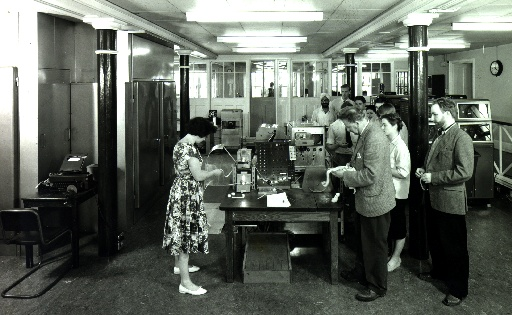
\includegraphics[width=1\textwidth]{imgs/EDSAC_2_1960.jpg}}
\end{frame}
\begin{frame}{Using HPC: Job Submission}
\begin{itemize}
\item{Compute resources are managed by a scheduler:\hfill\\\qquad\alert{SLURM}/PBS/SGE/LSF/\ldots}
\item{Jobs are submitted to the scheduler\hfill\\\qquad --- analogous to submitting jobs to a print queue\hfill\\\qquad --- a file (\emph{submission script}) is copied and queued\hfill\\\qquad \hphantom{---} for processing.}
\end{itemize}
\end{frame}

\begin{frame}{Using HPC: Job Submission}
\begin{itemize}
\item{Jobs are submitted from the \alert{login node}\hfill\\\qquad  --- not itself managed by the scheduler.}
\item{Jobs may be either non-interactive (\alert{batch}) or \alert{interactive}.}
\pause
\item{\alert{Batch} jobs run a shell script on the first of a list of allocated nodes.}
\item{\alert{Interactive} jobs provide a command line on the first of a list of allocated nodes.}
\end{itemize}
\end{frame}

\begin{frame}{Using HPC: Job Submission}
\begin{itemize}
\item{Jobs may use \alert{part} or \alert{all} of one or more nodes\hfill\\
\qquad --- the owner can specify \mbox{\tt --exclusive} to force exclusive\hfill\\\qquad\hphantom{---} node access (automatic on KNL).}
\item{Template submission scripts are available under\hfill\\
\qquad \alert{/usr/local/Cluster-Docs/SLURM}.}
\end{itemize}
\end{frame}

\begin{frame}[fragile]{Job Submission: Using SLURM}
\begin{itemize}
\item{Prepare a shell script and submit it to SLURM:}
\begin{semiverbatim}
\scriptsize
[abc123@login-e-1]$ sbatch slurm_submission_script
Submitted batch job {\color{red}790299}
\end{semiverbatim}
\end{itemize}
\end{frame}

\begin{frame}[fragile]{Job Submission: Show Queue}
\begin{itemize}
\item{Submitted job scripts are copied and stored in a queue:}
\begin{semiverbatim}
\tiny
[abc123@login-e-1]$ squeue -u abc123
             JOBID PARTITION     NAME     USER ST       TIME  NODES NODELIST(REASON)
            {\color{red}790299}   skylake     Test3  abc123 PD       0:00      2 (\only<1>{{\color{blue}Priority}}\only<2>{{\color{green}Resources}}\only<3>{{\color{red}AssocGrpCPUMinsLimit}})
            790290   skylake     Test2  abc123  R   27:56:10      2 cpu-e-[1,10]
\end{semiverbatim}
\end{itemize}
\end{frame}

\begin{frame}[fragile]{Job Submission: Monitor Job}
\begin{itemize}
\item{Examine a particular job:}
\begin{semiverbatim}
\scriptsize
[abc123@login-e-1]$ scontrol show job={\color{red}790290}
\end{semiverbatim}
\end{itemize}
\end{frame}

\begin{frame}[fragile]{Job Submission: Accounting Commands}
\begin{itemize}
\item{How many core hours available do I have?}
\begin{semiverbatim}
\tiny
mybalance

User           Usage |        Account     Usage | Account Limit Available (hours)
---------- --------- + -------------- --------- + ------------- ---------
sjr20              3 |    SUPPORT-CPU     2,929 |    22,425,600 {\color{red}22,422,671}
sjr20              0 |    SUPPORT-GPU         0 |        87,600    {\color{red}87,600}
\end{semiverbatim}
\smallskip
\item{How many core hours does some other project or user have?}
\begin{semiverbatim}
\tiny
gbalance -p SUPPORT-CPU

User           Usage |        Account     Usage | Account Limit Available (hours)
---------- --------- + -------------- --------- + ------------- ---------

pfb29          2,925 |    SUPPORT-CPU     2,929 |    22,425,600 22,422,671
sjr20 *            3 |    SUPPORT-CPU     2,929 |    22,425,600 22,422,671
...
(Use -u for user.)
\end{semiverbatim}
\smallskip
\item{List all jobs charged to a project/user between certain times:}
\begin{semiverbatim}
\Tiny
gstatement -p SUPPORT-CPU  -u xyz10 -s "2018-04-01-00:00:00" -e "2018-04-30-00:00:00" 
       JobID      User    Account    JobName  Partition                 End ExitCode      State  CompHrs 
------------ --------- ---------- ---------- ---------- ------------------- -------- ---------- -------- 
263              xyz10 support-c+ _interact+    skylake 2018-04-18T19:44:40      0:0    TIMEOUT      1.0
264              xyz10 support-c+ _interact+    skylake 2018-04-18T19:48:07      0:0 CANCELLED+      0.1
275              xyz10 support-c+ _interact+    skylake             Unknown      0:0    RUNNING      0.3
...
\end{semiverbatim}
\end{itemize}
\end{frame}


\begin{frame}[fragile]{Job Submission: Cancel Job}
\begin{itemize}
\item{Cancel a particular job:}
\begin{semiverbatim}
\scriptsize
[abc123@login-e-1]$ scancel {\color{red}790290}
\end{semiverbatim}
\end{itemize}
\end{frame}

\begin{frame}[fragile]{Job Submission: Scripts}
\begin{itemize}
\item{SLURM\hfill\\
In \alert{/usr/local/Cluster-Docs/SLURM, see examples: \alert{slurm\_submit.peta4-skylake}, \alert{slurm\_submit.wilkes2}.}
  
\begin{semiverbatim}
\tiny
#!/bin/bash
#! Name of the job:
{\color<2->{red}#SBATCH} -J myjob
#! Which project should be charged:
{\color<2->{red}#SBATCH} -A CHANGEME
#! How many whole nodes should be allocated?
{\color<2->{red}#SBATCH} --nodes=1
#! How many tasks will there be in total? (<= nodes*32)
{\color<2->{red}#SBATCH} --ntasks={\color<3->[rgb]{1,0,0}\only<1-3>{1}\only<4->{16}}
#! How much wallclock time will be required?
{\color<2->{red}#SBATCH} --time=02:00:00
#! Select partition:
{\color<2->{red}#SBATCH} -p skylake
...
\end{semiverbatim}}
\item<2->{{\color{red}\#SBATCH} lines are \emph{structured comments}\hfill\\
\qquad --- correspond to sbatch command line options.}
\item<3->{\alert{The above job will be given {\color<3->[rgb]{1,0,0}\only<1-3>{1 cpu}\only<4->{16 cpus}} on 1 node for 2 hours (by default there is 1 task per node, and 1 cpu per task).}}
\end{itemize}
\end{frame}

\subsection{Single Node Jobs}
\begin{frame}[fragile]{Job Submission: Single Node Jobs}
\begin{itemize}
\item{Serial jobs requiring large memory, or OpenMP codes.}
\begin{semiverbatim}
\scriptsize
#!/bin/bash
\ldots
#SBATCH --nodes=1
\uncover<2-|handout:2->{{\color{red}#SBATCH --ntasks=1
# Default is 1 task per node}} 
\uncover<3-|handout:2->{{\color{red}#SBATCH --cpus-per-task=\only<3-5|handout:2>{1}\only<6,8-|handout:3,5->{32 # Whole node}\only<7|handout:4>{16  # Half node}
\only<3-5|handout:2>{# Default is 1 cpu (core) per task}}}
\uncover<4-5|handout:2>{{\color{red}#SBATCH --mem=5990
# Memory per node in MB - default is pro rata by cpu number}}
\uncover<5|handout:2>{{\color{red}# Increasing --mem or --cpus-per-task implicitly increases the other}}
\ldots
\uncover<6-|handout:3->{{\color{red}export OMP\_NUM\_THREADS=\only<6|handout:3>{32}\only<7-|handout:4->{16}  # For OpenMP across \only<6|handout:3>{32}\only<7-|handout:4->{16} cores\only<8-|handout:5->{ (using all memory)}}}
$application \$options
\ldots
\end{semiverbatim}
\end{itemize}
\end{frame}

\subsection{MPI Jobs}
\begin{frame}[fragile]{Job Submission: MPI Jobs}
\begin{itemize}
\item{Parallel job across multiple nodes.}
\begin{semiverbatim}
\scriptsize
#!/bin/bash
\ldots
#SBATCH --nodes={\color{red}4}
#SBATCH --ntasks=\alert{\only<1|handout:1>{128}\only<2-|handout:2->{64}}     # \only<1|handout:1>{i.e.\ {\color[rgb]{0,0.8,0}32}}\only<2-|handout:2->{i.e.\ {\color[rgb]{0,0.8,0} 16}}x{\color{red}4} MPI tasks in total.
\uncover<2-|handout:2->{{\color{red}#SBATCH --cpus-per-task=2}}
\ldots
mpirun\only<2-|handout:2->{ -ppn {\color[rgb]{0,0.8,0}16}} -np \alert{\only<1|handout:1>{128}\only<2-|handout:2->{64}} \$application \$options
\ldots
\end{semiverbatim}
\item<3-|handout:2->{\small \alert{SLURM-aware MPI} launches remote tasks via SLURM (doesn't need a list of nodes).}
%\item<3-|handout:2->{\small The template script uses \$SLURM\_TASKS\_PER\_NODE to set PPN.}
\end{itemize}
\end{frame}

\subsection{Hybrid Jobs}
\begin{frame}[fragile]{Job Submission: Hybrid Jobs}
\begin{itemize}
\item{Parallel jobs using both MPI and OpenMP.}
\begin{semiverbatim}
\scriptsize
#!/bin/bash
\ldots
#SBATCH --nodes={\color{red}4}
#SBATCH --ntasks=\alert{64}     # i.e.\ {\color[rgb]{0,0.8,0}16}x{\color{red}4} MPI tasks in total.
#SBATCH --cpus-per-task={\color{brown}2}
\ldots
{\color{brown}export OMP\_NUM\_THREADS=2   # i.e.\ 2 threads per MPI task.}
mpirun -ppn {\color[rgb]{0,0.8,0}16} -np \alert{64} \$application \$options
\ldots
\end{semiverbatim}
\item<2->{\small This job uses \alert{128 CPUs} (each MPI task splits into 2 OpenMP threads).}
\end{itemize}
\end{frame}

\subsection{High Throughput Jobs}
\begin{frame}[fragile]{Job Submission: High Throughput Jobs}
\begin{itemize}
\item{Multiple serial jobs across multiple nodes.}
\item{Use \alert{srun} to launch tasks (\alert{job steps}) within a job.}
\begin{semiverbatim}
\scriptsize
#!/bin/bash
\ldots
#SBATCH --nodes=2
\ldots
cd directory\_for\_job1
\alert{srun} {\color<3>{red}--exclusive} {\color<2>{red}-N 1 -n 1} \$application \$options\_for\_job1 > output 2> err {\color<4>{red}&}
cd directory\_for\_job2
\alert{srun} {\color<3>{red}--exclusive} {\color<2>{red}-N 1 -n 1} \$application \$options\_for\_job2 > output 2> err {\color<4>{red}&}
...
cd directory\_for\_job64
\alert{srun} {\color<3>{red}--exclusive} {\color<2>{red}-N 1 -n 1} \$application \$options\_for\_job64 > output 2> err {\color<4>{red}&}
{\color<5>{red}wait}
\end{semiverbatim}
\item<6>{Exercise 6--8 - Submitting Jobs.}
\end{itemize}
\end{frame}

\subsection{Interactive Jobs}
\begin{frame}[fragile]{Job Submission: Interactive}
\begin{itemize}
\item{Compute nodes are accessible via SSH \alert{while you have a job running on them}.}
\pause
\item{Alternatively, submit an interactive job:}
\begin{semiverbatim}
\alert{sintr -A TRAINING-CPU -N1 -n8 -t 1:0:0}
\end{semiverbatim}
\medskip
\pause
\item{Within the window (screen session):}
\begin{itemize}
\item[$\ast$]{Launches a shell on the first node (when the job starts).}
\item[$\ast$]{Graphical applications should display correctly \alert{(if they did from the login node)}.}
\item[$\ast$]{Create new shells with \alert{ctrl-a c}, navigate with \alert{ctrl-a n} and \alert{ctrl-a p}.}
\item[$\ast$]{\alert{ssh} or \alert{srun} can be used to start processes on any nodes in the job.}
\item[$\ast$]{SLURM-aware MPI will do this automatically.}
\end{itemize}
\end{itemize}
\end{frame}


\subsection{Array Jobs}
\begin{frame}[fragile]{Job Submission: Array Jobs}
\begin{itemize}
\item{\alert{$http://slurm.schedmd.com/job\_array.html$}}
\item{Used for submitting and managing large sets of similar jobs.}
\item{Each job in the array has the same \alert{initial} options.}
\item{SLURM}
\begin{semiverbatim}
\scriptsize
[abc123@login-e-1]$ sbatch --array=\only<1,2>{{\color{red}1-7}}\only<2>{{\color{red}:2}}\only<3->{{\color{red}1,3,5,7}} -A TRAINING-CPU submit\_script
Submitted batch job {\color[rgb]{0,0.6,0}791609}
\tiny
\uncover<4->{[abc123@login-e-1]$ squeue -u abc123
             JOBID PARTITION     NAME     USER ST       TIME  NODES NODELIST(REASON)
          {\color[rgb]{0,0.6,0}791609}\_{\color{red}1} skylake      hpl    abc123  R       0:06      1 cpu-a-6
          {\color[rgb]{0,0.6,0}791609}\_{\color{red}3} skylake      hpl    abc123  R       0:06      1 cpu-a-16
          {\color[rgb]{0,0.6,0}791609}\_{\color{red}5} skylake      hpl    abc123  R       0:06      1 cpu-a-7
          {\color[rgb]{0,0.6,0}791609}\_{\color{red}7} skylake      hpl    abc123  R       0:06      1 cpu-a-7
}
\end{semiverbatim}
\uncover<5->{\centerline{{\color[rgb]{0,0.6,0}791609}\_{\color{red}1}, {\color[rgb]{0,0.6,0}791609}\_{\color{red}3}, {\color[rgb]{0,0.6,0}791609}\_{\color{red}5}, {\color[rgb]{0,0.6,0}791609}\_{\color{red}7}}}
\smallskip
\uncover<6->{\centerline{i.e.\ \$\{{\color[rgb]{0,0.6,0}SLURM\_ARRAY\_JOB\_ID}\}\_\$\{{\color{red}SLURM\_ARRAY\_TASK\_ID}\}}}
\smallskip
\uncover<7->{\leftline{\small SLURM\_ARRAY\_JOB\_ID${}={}$SLURM\_JOBID for the first element.}}
\end{itemize}
\end{frame}

\begin{frame}[fragile]{Job Submission: Array Jobs (ctd)}
\begin{itemize}
\item{Updates can be applied to specific array elements using \$\{{\color[rgb]{0,0.6,0}SLURM\_ARRAY\_JOB\_ID}\}\_\$\{{\color{red}SLURM\_ARRAY\_TASK\_ID}\}}
\item{Alternatively operate on the entire array via \$\{{\color[rgb]{0,0.6,0}SLURM\_ARRAY\_JOB\_ID}\}}.
\item{Some commands still require the SLURM\_JOB\_ID (sacct, sreport, sshare, sstat and a few others).}
\pause
\item{Exercise 9 - Array Jobs.}
\end{itemize}
\end{frame}

\subsection{Scheduling}
\begin{frame}{Scheduling}
\begin{itemize}
\item{SLURM scheduling is multifactor:}
  \pause
\begin{itemize}
\item{\alert{QoS} --- payer or non-payer?}
  \pause
\item{\alert{Age} --- how long has the job waited?\hfill\\\qquad
  \alert{Don't cancel jobs that seem to wait too long.}}
  \pause
\item{\alert{Fair Share} --- how much recent usage?\hfill\\\qquad
  \alert{Payers with little recent usage receive boost.}}
  \pause
\item{\alert{sprio -j jobid}}
\end{itemize}
\pause
\item{\alert{Backfilling}}
\begin{itemize}
  \item{Promote lower priority jobs into gaps left by higher priority jobs.}
    \item{Demands that the higher priority jobs not be delayed.}
    \item{Relies on reasonably accurate wall time requests for this to work.}
      \item{Jobs of default length will not backfill readily.}
\end{itemize}
\end{itemize}
\end{frame}

\subsection{Wait Times}
\begin{frame}{Wait Times}
  \begin{itemize}
  \item{36 hour job walltimes are permitted.}
    \pause
  \item{\alert{This sets the timescale at busy times (\emph{without} backfilling).}}
    \pause
  \item{Use backfilling when possible.}
  \item{Short (1 hour or less) jobs have higher throughput.}
\end{itemize}
\end{frame}

\subsection{Checkpointing}
\begin{frame}{Checkpointing}
  \begin{itemize}
  \item{Insurance against failures during long jobs.}
  \item{Restart from checkpoints to work around finite job length.}
    \pause
  \item{Application native methods are best. Failing that, one can try \alert{DMTCP}:\hfill\break
  \null\qquad \alert{http://dmtcp.sourceforge.net/index.html}}
  \end{itemize}
\end{frame}

\subsection{Scheduling Top Tips}
\begin{frame}{Job Submission: Scheduling Top Dos \& Don'ts}
\begin{itemize}
\item{\textbf{Do \ldots}}
\begin{itemize}
\item{Give reasonably accurate wall times (allows \alert{backfilling}).}
\item{Check your balance occasionally (\alert{mybalance}).}
\item{Test on a small scale first.}
\item{Implement \alert{checkpointing} if possible (reduces resource wastage).}
\end{itemize}
\medskip
\item{\textbf{Don't \ldots}}
\begin{itemize}
\item{Request more than you need\hfill\\
\qquad --- you will wait longer and use more credits.}
\item{Cancel jobs unnecessarily\hfill\\
\qquad ---  priority increases over time.}
\end{itemize}
\end{itemize}
\end{frame}



\end{document}
